\chapter{Fejlesztői dokumentáció} 
\label{ch:impl}

Az alkalmazás \textbf{Microsoft Visual Studio} segítségével készült. A kódok elsősorban C++, másodsorban -- a shaderek -- GLSL nyelven íródtak. Ha újra akarnánk fordítani akkor a \textbf{C:/} helyre csomagoljuk ki a mellékelt \textbf{OGLPack.zip} állományt (ez az szükséges csomagokat és függőségeket tartalmazza), majd futtassuk a \textbf{subst T: C:/} parancsot. Ezután megnyithatjuk a \textbf{.vcxproj} kiterjesztésű projektfájlt.

\section{Fejlesztői eszközök}

A program írása során számos könyvtár és API felhasználásra került. Ebben az alfejezetben ezek kerülnek bemutatásra.

\subsubsection{Simple DirectMedia Layer (SDL)}
A Simple DirectMedia Layer (SDL) könyvtár egy crossplatform multimédiás könyvtár, ami alacsony szintű, hatékony hozzáférést ad audio, bemeneti (egér, billentyűzet, joystick), valamint grafikus (OpenGL-en keresztül GPU-hoz) eszközökhöz. Az alkalmazásban az SDL 2.0 van használva. \cite{SimpleDi88:online}

\begin{figure}[H]
	\centering
	
\includegraphics[width=0.5\textwidth]{Sdl}
	\caption{Az SDL logója}
	\label{fig:Sdl}
\end{figure}

\subsubsection{OpenGL API}
Az OpenGL (Open Graphics Library) egy részletesen kidolgozott szabvány, melyet a Silicon Graphics nevű amerikai cég fejlesztett ki 1992-ben. Olyan API-t takar, amely segítségével egy egyszerű, szabványos felületen keresztül megvalósítható a grafikus kártya kezelése és a háromdimenziós grafika programozása. Az interfész több ezer különböző függvényhívásból áll, melynek segítségével a programozók szinte közvetlenül vezérelhetik a grafikus kártyát, segítségükkel 3 dimenziós alakzatokat rajzolhatnak ki, és a kirajzolás módját szabályozhatják. \cite{OpenGL–W93:online} 

\begin{figure}[H]
	\centering
	
\includegraphics[width=0.5\textwidth]{Opengl}
	\caption{Az OpenGL logója}
	\label{fig:Opengl}
\end{figure}

\subsubsection{Dear ImGui}
A \textbf{``Parameters''} feliartú panel megjelenítése ennek segítségével lett megoldva. A Dear ImGui (ImGui) egy egyszerű grafikai interfész könyvtár C++ nyelvhez. Segítségével egyszerűen kezelhetünk gombokat, csúszkákat, egyéb beviteli eszközöket valamint könnyen megjeleníthetünk adatokat. Gyors és hordozható, nincs szükség külső könyvtárra csak néhány szimpla forrásfájl beillesztésére. \cite{ocornuti13:online}

\subsubsection{GLM}

Az OpenGL Mathematics egy headerben importálható C++ könyvtár mely a GLSL specifikációira szabva (elnevezések, funkciók) tartalmaz számtalan matematikai függvényt. Segítségével a GLSL-ben használatos függvények és típusok C++-ban is használhatóak. \cite{OpenGLMa34:online}

\begin{figure}[H]
	\centering
	\includegraphics[width=0.5\textwidth]{GLM}
	\caption{A GLM logója}
	\label{fig:GLM}
\end{figure}

\section{Képalkotási módszer}
\label{sec:kepmod}

A megjelenítés \textbf{Raycast} technika (\ref{fig:trace_diag}.~ábra) alkalmazásával történik, egy speciális implicit reprezentáción: a távolságfüggvényeken. Ehhez minden pixelre ki kell számolni egy sugár paramétereit. Ezen sugár és felület metszetét a \textbf{Sphere tracing} algoritmussal kapjuk meg. A felületi normálist numerikusan számítjuk ki, melynek segítségével a felület már könnyen árnyalható.

\begin{figure}[H]
	\centering
	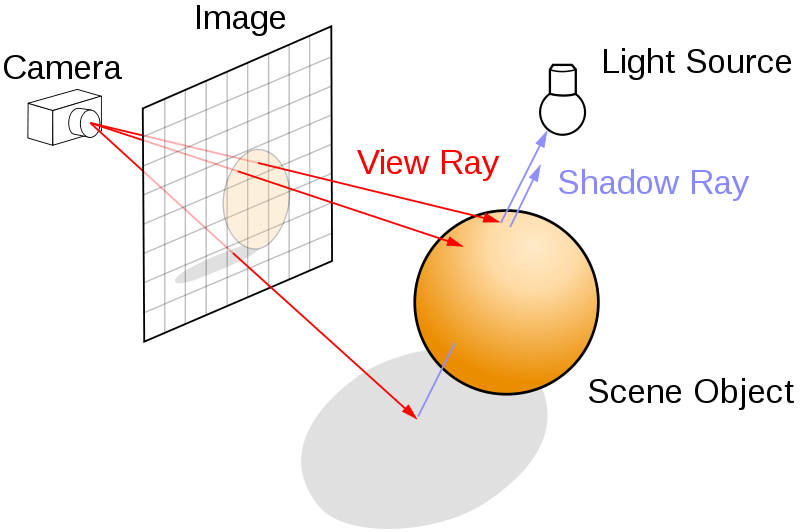
\includegraphics[width=0.5\textwidth]{trace_diag}
	\caption{A raycast technika ábrázolása. \cite{FileRayt97:online}}
	\label{fig:trace_diag}
\end{figure}

A \textbf{sphere tracing} algoritmus egy speciális esete az úgynevezett \textbf{raymarching} algoritmus-családnak. Működéséhez a kirajzolni kívánt objektumokat távolságfüggvényekkel kell reprezentálni, mely a virtuális tér bármely pontjáról képes meghatározni hogy milyen messze van az objektum felületétől. Az algoritmus egy implementációja \aref{src:raymarch}. forráskód részletben látható.

\lstset{caption={A sphere tarcing algoritmust megvalósító kód}, label=src:raymarch}
\begin{lstlisting}[language={C}]
float RayMarch(vec3 ro, vec3 rd) {
	float dist=0.0;    
    for(int i=0; i<MAX_STEPS; i++) {
        vec3 p = ro + rd*dist;
        float dS = GetDist(p);
        dist += dS;
        if(dist>MAX_DIST || dS<SURF_DIST ) break;
    }    
    return dist;
}
\end{lstlisting}

Az algoritmus két paramétert igényel: egy pontot (\textbf{ro}) és egy vektort (\textbf{rd}), melyek meghatározzák a sugár kezdőpontját és irányát. Ezen irány mentén lépked folyamatosan mindig annyit, amennyi amekkora a távolság a legközelebbi felülethez képest. Ezt addig csinálja míg már kellően közel lesz (dS<SURF\_DIST), vagy ha már túl messzire ment (dist>MAX\_DIST), vagy esetleg túl sokat lépett (i>MAX\_STEP). 


\begin{figure}[H]
	\centering
	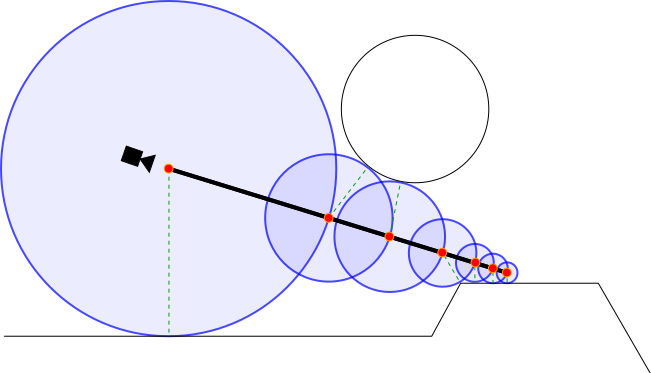
\includegraphics[width=0.4\textwidth]{SphereTracing}
	\caption{Sphere tracing: A kamerából kiinduló fénysugár mindig csak annyit halad előre amekkora a hozzá legközelebb lévő felület távolsága \cite{Raymarch94:online}}
	\label{fig:SphereTracing2}
\end{figure}

Az alkalmazásban teljesítményjavítás érdekében másik feltétel (dS<0.01*dist/MAX\_DIST) lett használva a felületi távolsághoz, mely számításba veszi hogy mennyire messzire vagyunk a kamerától. Ha messzebb vagyunk akkor nincsen szükség akkora részletességre és a felületi távolság így lehet nagyobb is.

\subsection{Fénymodell}
\label{sec:lighting}
Ha túl messzire ment a sugarunk (dist>MAX\_DIST), akkor egyszerűen a háttér színét adjuk a pixelnek. Egyéb esetben pedig kiszámoljuk az adott pontban a felületi normálist és a fénymodell segítségével megállapítjuk a pixel színét.

A használt fénymodell nagyon sokat számít a kirajzolt kép minőségén. Ezért sok idő és energia lett rászánva ennek megalkotására, a végeredményre Ingio Quilez munkássága \cite{iqShader82:online} nagy befolyást gyakorlot. Ezen fénymodell komponensei \aref{fig:lighting}.~ábrán láthatóak. Ezek különböző színenkénti súlyozással vett összege alkotja a végső színáranyalatot, melyre még egy gamma korrekció és egy ködszerű hatás is alkalmazva lett -- ez utóbbi arra szolgál hogy a viszonylag kicsi maximális távolságot leplezze.

\begin{figure}[H]
	\centering
	\subfigure[Objektumok alapszíne]{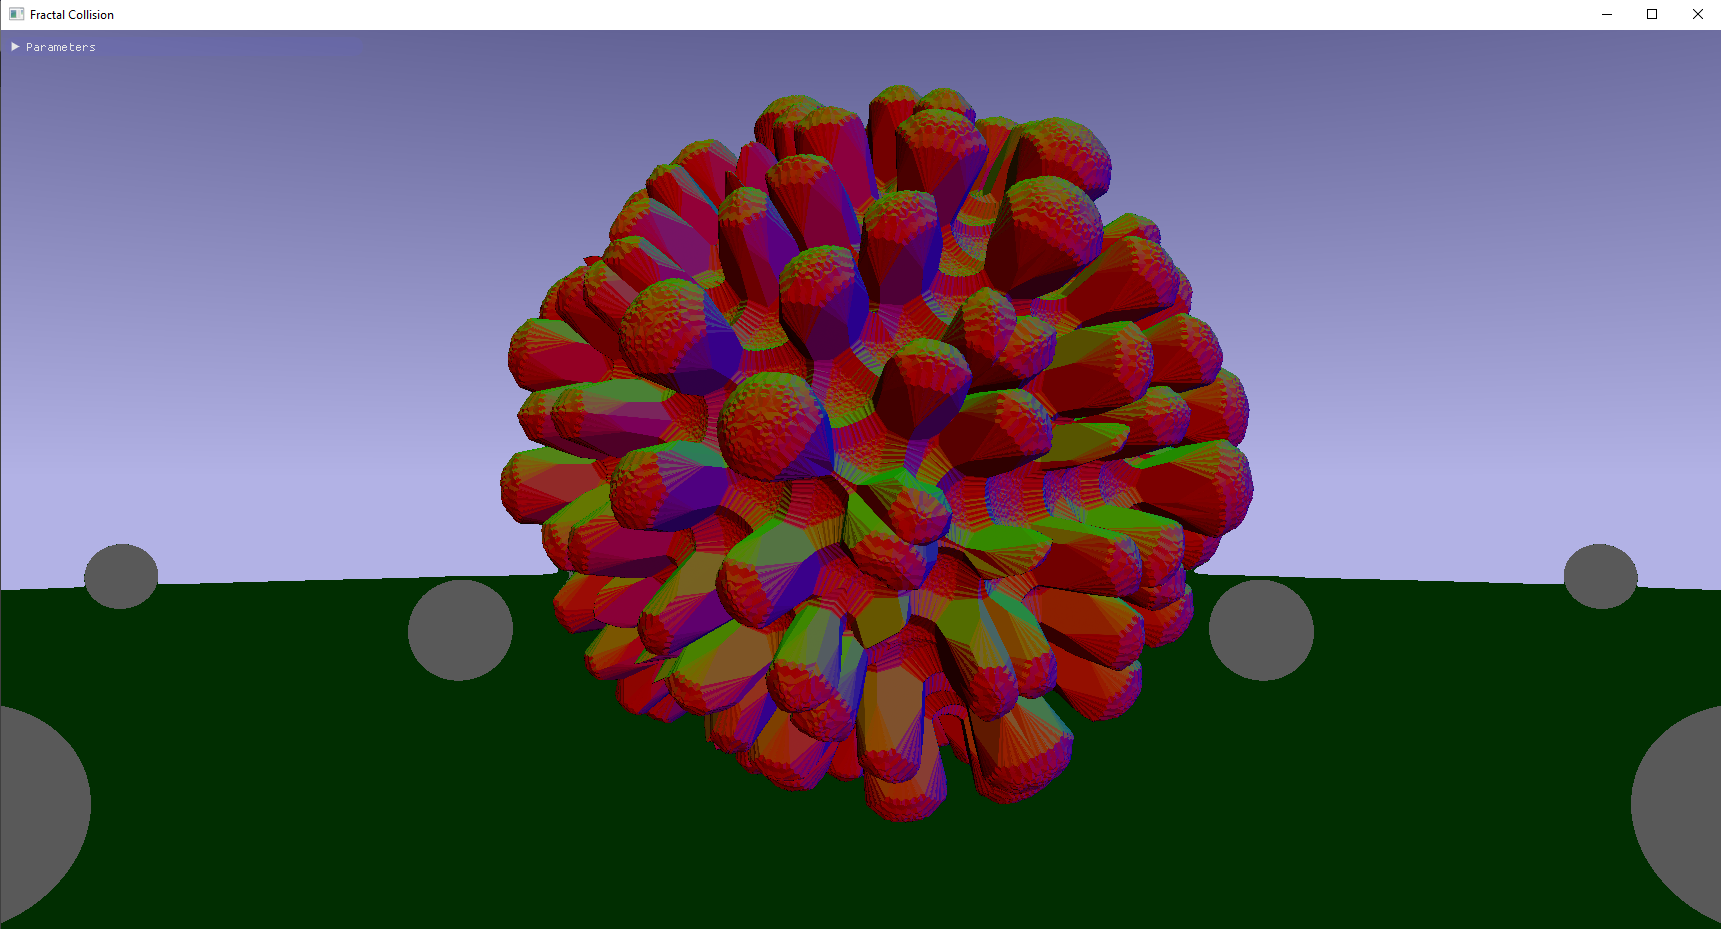
\includegraphics[width=0.3\linewidth]{col}}
	\hspace{1pt}
	\subfigure[Módosított ambiens fény]{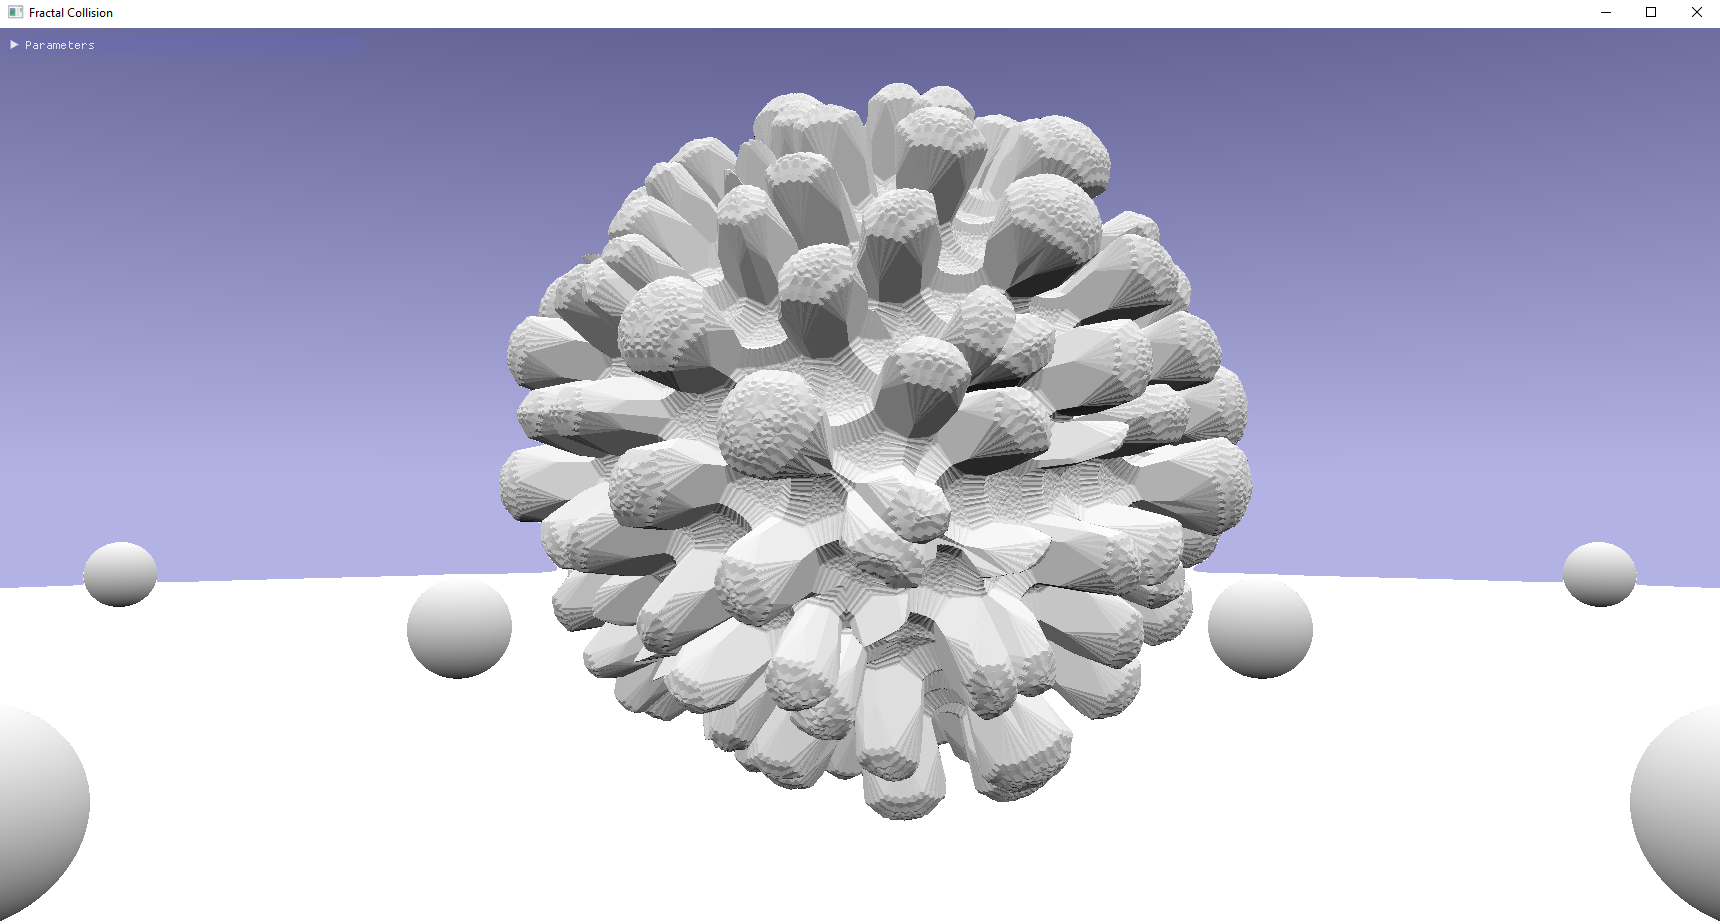
\includegraphics[width=0.3\linewidth]{amb}}
	\hspace{1pt}
	\subfigure[Ambiens eltakarás]{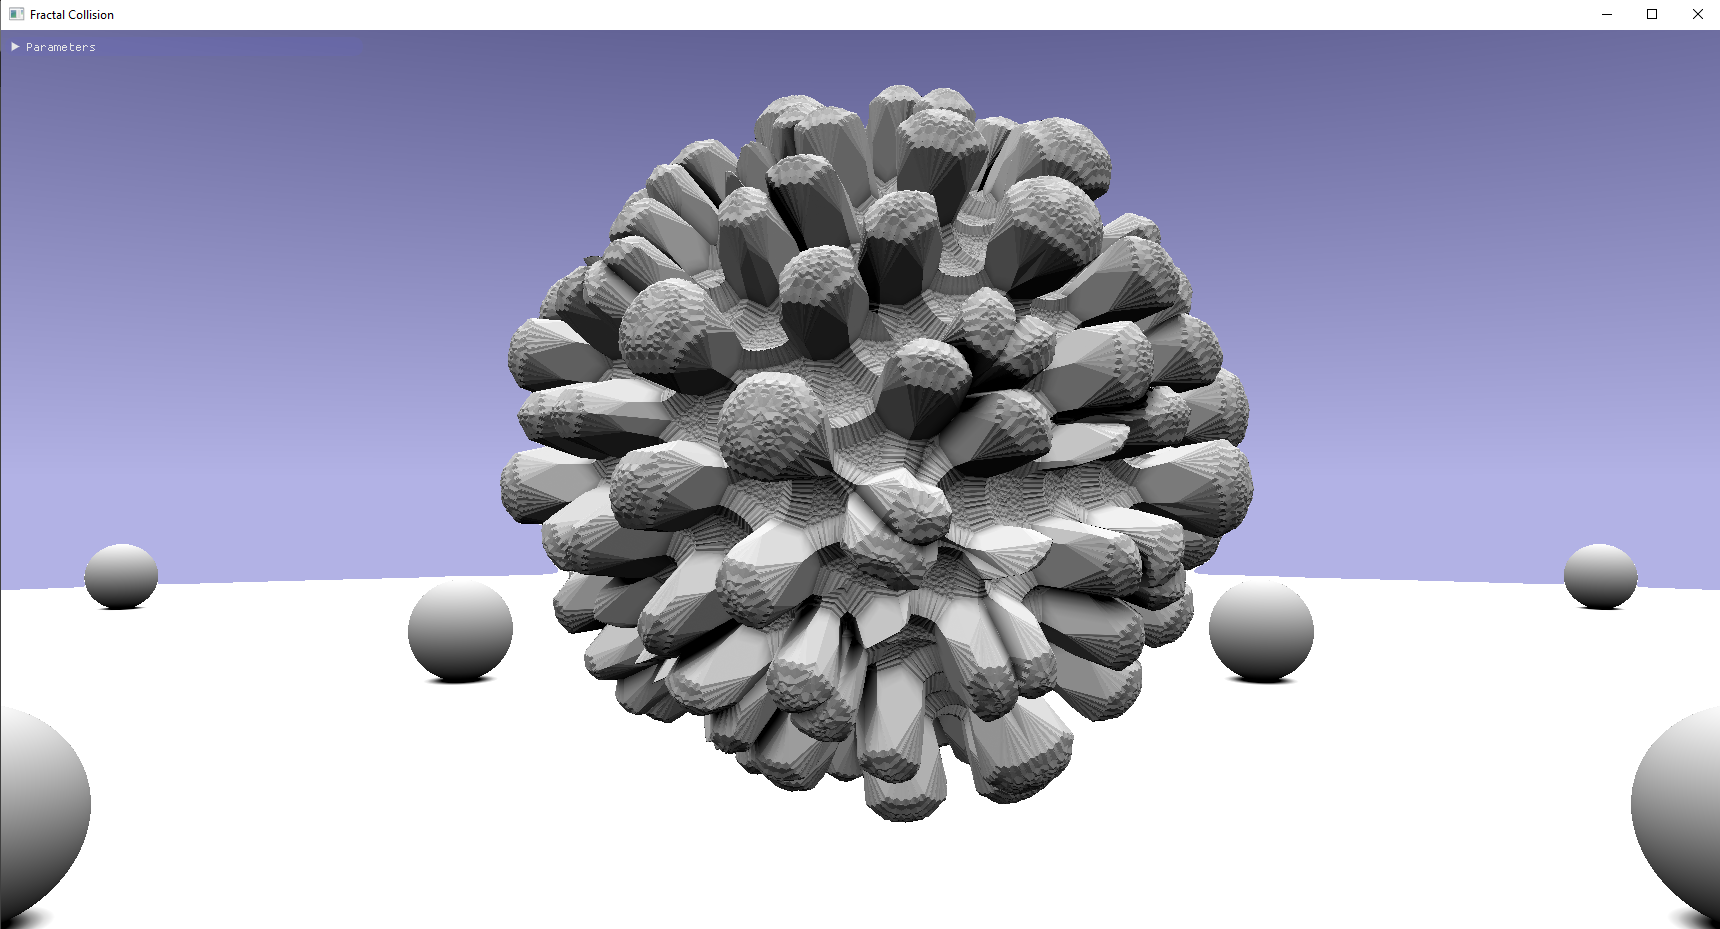
\includegraphics[width=0.3\linewidth]{occ}}
	\vspace{1pt}
	\subfigure[Spekuláris]{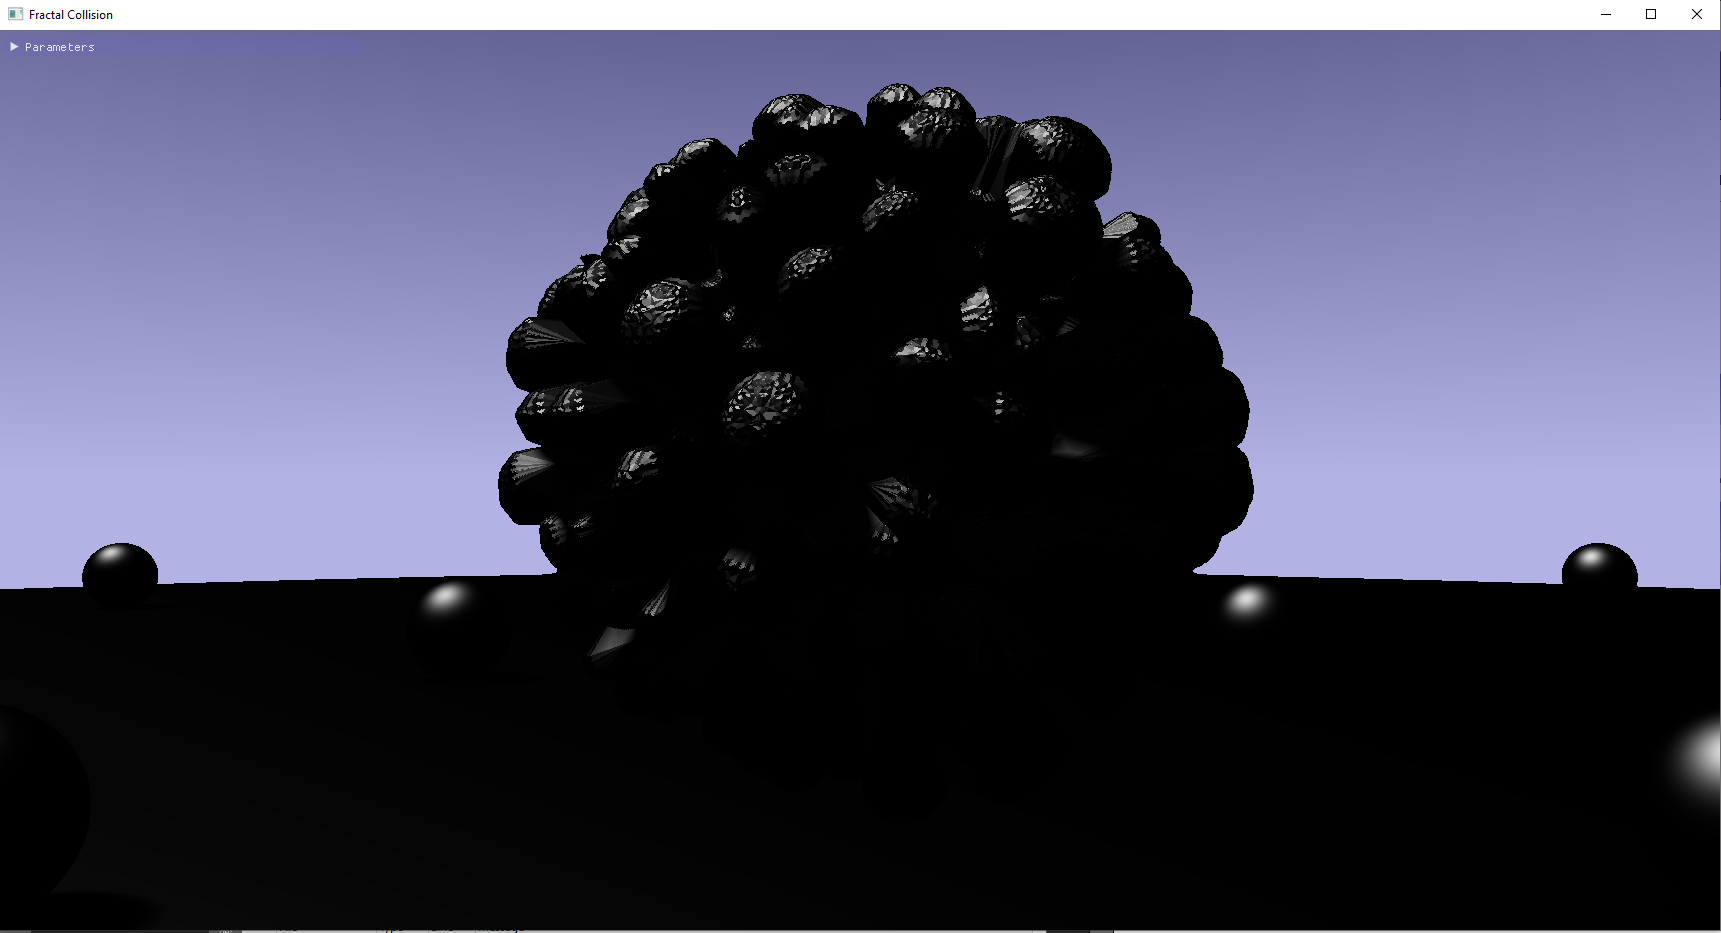
\includegraphics[width=0.3\linewidth]{spe}}
	\hspace{1pt}
	\subfigure[Diffúz * Árnyék]{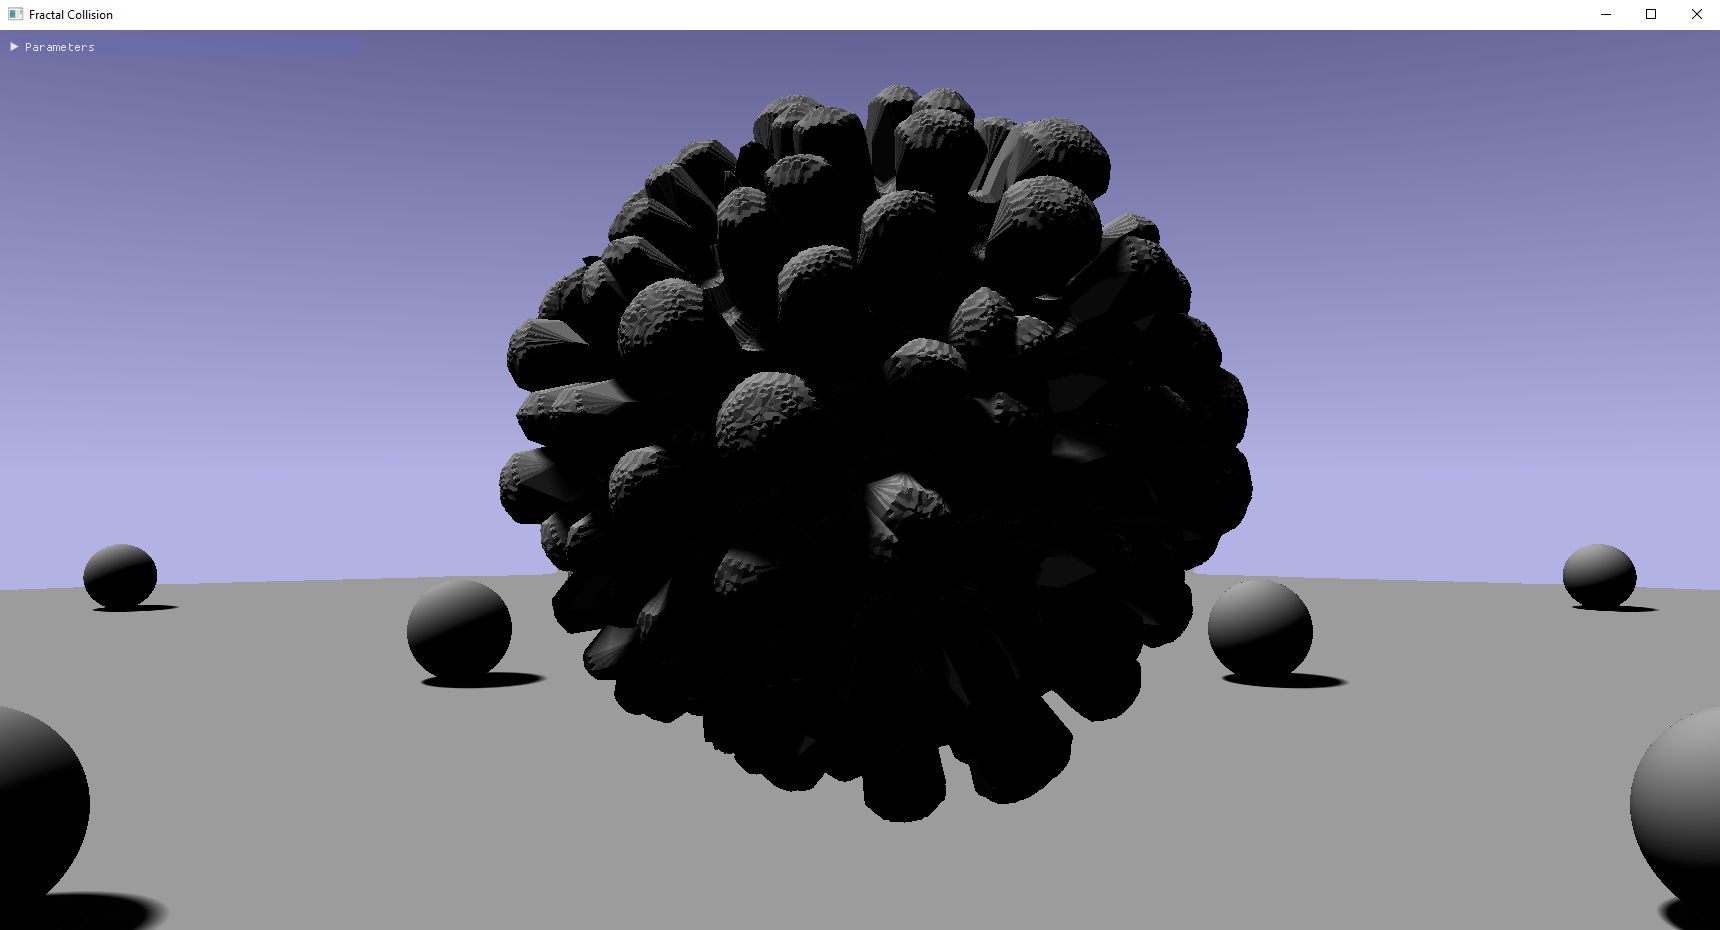
\includegraphics[width=0.3\linewidth]{shadif}}
	\hspace{1pt}
	\subfigure[Ellenfény]{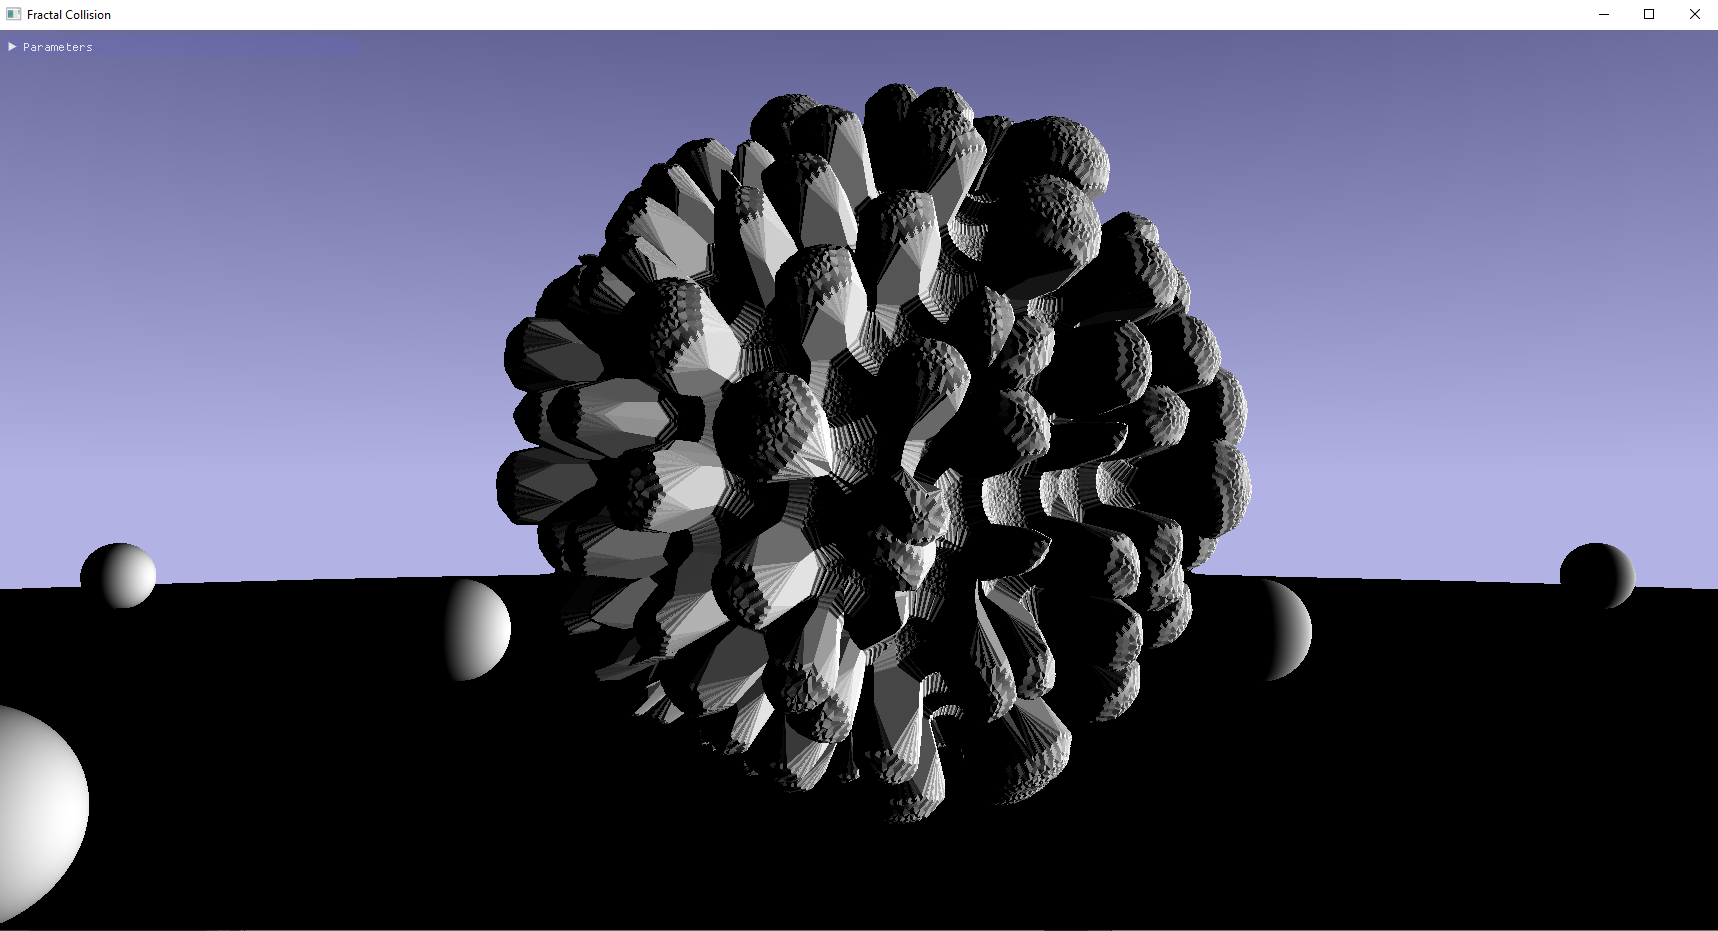
\includegraphics[width=0.3\linewidth]{bac}}
	\vspace{1pt}
	\subfigure[Élfény]{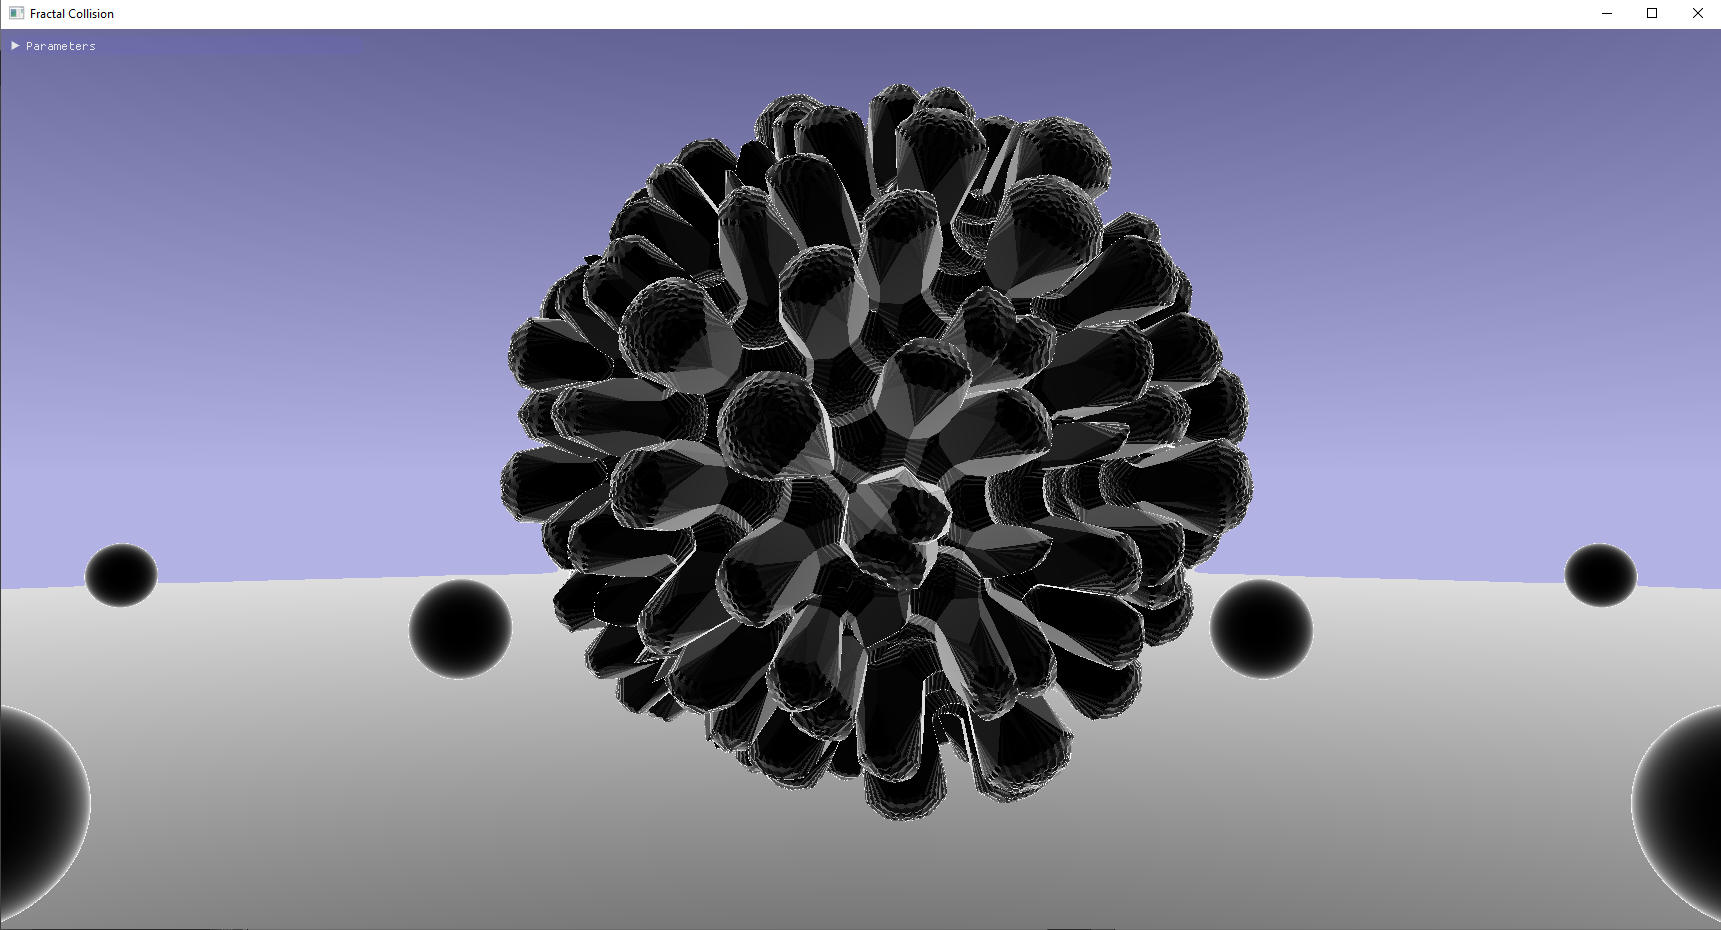
\includegraphics[width=0.3\linewidth]{fre}}
	\hspace{1pt}
	\subfigure[Árnyékalapú tükröződés]{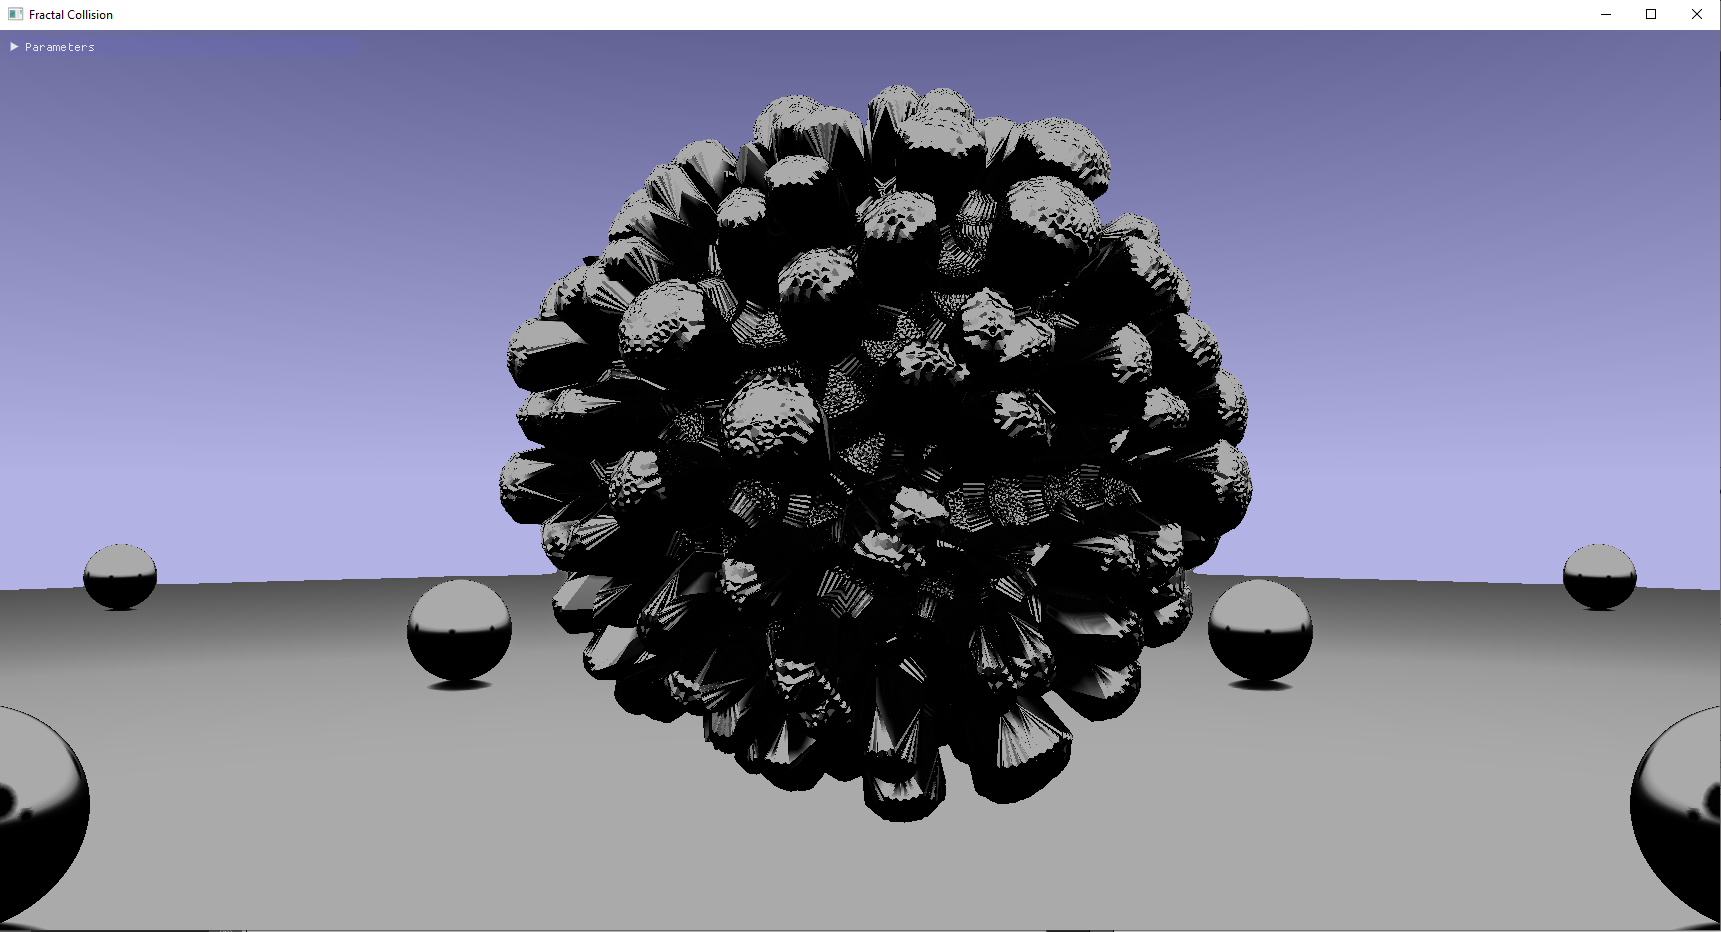
\includegraphics[width=0.3\linewidth]{shadom}}	
	\caption{A fénymodell különböző komponensei.}
	\label{fig:lighting}
\end{figure}

\subsection{Távolságfüggvények}

Távolságfüggvényekkel reprezentáljuk az objketumokat. Ebből adódóan nagyon fontosak a megjelenítés szempontjából. Ebben az alfejezetben matematikai szempontból kerülnek részletesebb ismertetésre. A távolságfüggvények matematikai tárgyalását Bálint Csaba munkája \cite{Távolság48:online} alapján részletezzük.

\begin{definition}
Legyen az $(\mathbb{R}^{3}, d)$ metrikus térben egy $x  \in \mathbb{R}^{3}$ pont és egy $A \subset \mathbb{R}^{3}$ halmaz távolsága az alábbi:
\[
d(x, A):=\inf _{a \in A} d(x, a)
\]
\end{definition}

\begin{definition}
Az  $f: \mathbb{R}^{3} \rightarrow \mathbb{R}$  akkor távolságfüggvény, ha \\
$$\qquad f(\boldsymbol{p})=d\left(\boldsymbol{p},  \{f = 0\}\right) \quad\left(\boldsymbol{p} \in \mathbb{R}^{3}\right)$$
\end{definition}

Vagyis a távolságfüggvény az ábrázolni kívánt alakzat felületén 0 értéket vesz fel, mindenhol máshol pedig ettől a felülettől vett távolságot. Ennek egy kiterjesztése az \textbf{előjeles távolságfüggvény}, mely a távolságnak negatív előjelet ad az általa reprezentált alakzaton belül. Az alkamazásban ilyen távolságfüggvények kerültek felhasználásra. 

\begin{definition}
Az $f: \mathbb{R}^{3} \rightarrow \mathbb{R}$ pontosan akkor előjeles távolságfüggvény, ha létezik $D \subset \mathbb{R}^{3}$ halmaz, melyre
\[
f(\boldsymbol{p})=\left\{\begin{array}{ll}
d(\boldsymbol{p}, \text { bound }(D)) & \text { ha } \boldsymbol{p} \in D \\
-d(\boldsymbol{p}, \text { bound }(D)) & \text { ha } \boldsymbol{p} \notin D
\end{array}\right.
\]
ahol bound $(D)=\bar{D} \backslash \operatorname{int}(D)$ a halmaz határa.
\end{definition}

\cleardoublepage
Nagyon sok matematikai alakzatnak ismert az előjeles távolságfüggvénye. Az alkalmazásban csupán néhány egyszerűbb alakzat lett felhasználva:
$$\begin{array}{|l|l|l|}
\hline \text { Felület } & \text { Paraméterei } & \text { Előjeles távolságfüggvények } \\
\hline \text { Sík } & \begin{array}{l}
n \in \mathbb{R}^{3} \text { normális } \\
\|\boldsymbol{n}\|_{2}=1
\end{array} & f_{n}(\boldsymbol{p})=\langle\boldsymbol{p}, n\rangle \\
\hline \text { Gömb } & 0<r \in \mathbb{R} \text { sugár } & f_{r}(\boldsymbol{p})=\|\boldsymbol{p}\|_{2}-r \\
\hline \text { Téglatest } & \begin{array}{l}
a, b, c \in \mathbb{R} \\
\text {oldalhosszak}
\end{array} & \begin{array}{l}
\boldsymbol{d}:=\left[d_{x}, d_{y}, d_{z}\right]^{\top}:=\big[|x|-a,|y|-b,|z|-c\big]^{\top},\\
\text { ekkor } f_{a, b, c}(x, y, z)=\\
\min \left\{\max \left\{d_{x}, d_{y}, d_{z}\right\}, 0\right\}+\|\max \{\boldsymbol{d}, \boldsymbol{0}\}\|_{2}
\end{array} \\
\hline
\end{array}$$


Az előjeles távolságfüggvénnnyel leírt alakzatokkal könnyen végezhetünk műveleteket. Legyen $f, g \in \mathbb{R}^{3} \rightarrow \mathbb{R}$ előjeles távolságfüggvények. Ekkor megkapjuk az általuk leírt felületek \\
a) \textbf{unióját}, ha vesszük $f$ és $g$ minimumát \\
b) \textbf{metszetét}, ha vesszük $f$ és $g$ maximumát \\
c) \textbf{különbségét}, ha vesszük $f$ és $-g$ (vagy $-f$ és $g$) maximumát\\
Az így kapott függvények már csak előjeles távolságfüggvény-becslések lesznek. Ha egyszerre több alakzatot is ki akarunk rajzolni akkor a függvények unióját kell venni. Egy ilyen unió eredményét adja vissza a Sphere Tracing algoritmusban használt \textbf{GetDist()} eljárás. 

Továbbá ezen műveletekkel akár új alakzatot is alkothatunk! Például két koncentrikus gömb különbségéből ha kivonunk egy síkot akkor egy tál szerű alakzatatot kaphatunk (\ref{fig:bowl}. ábra), melyben kitűnően lehet tesztelni a labdák egymásnak ütközését.

\begin{figure}[H]
	\centering
	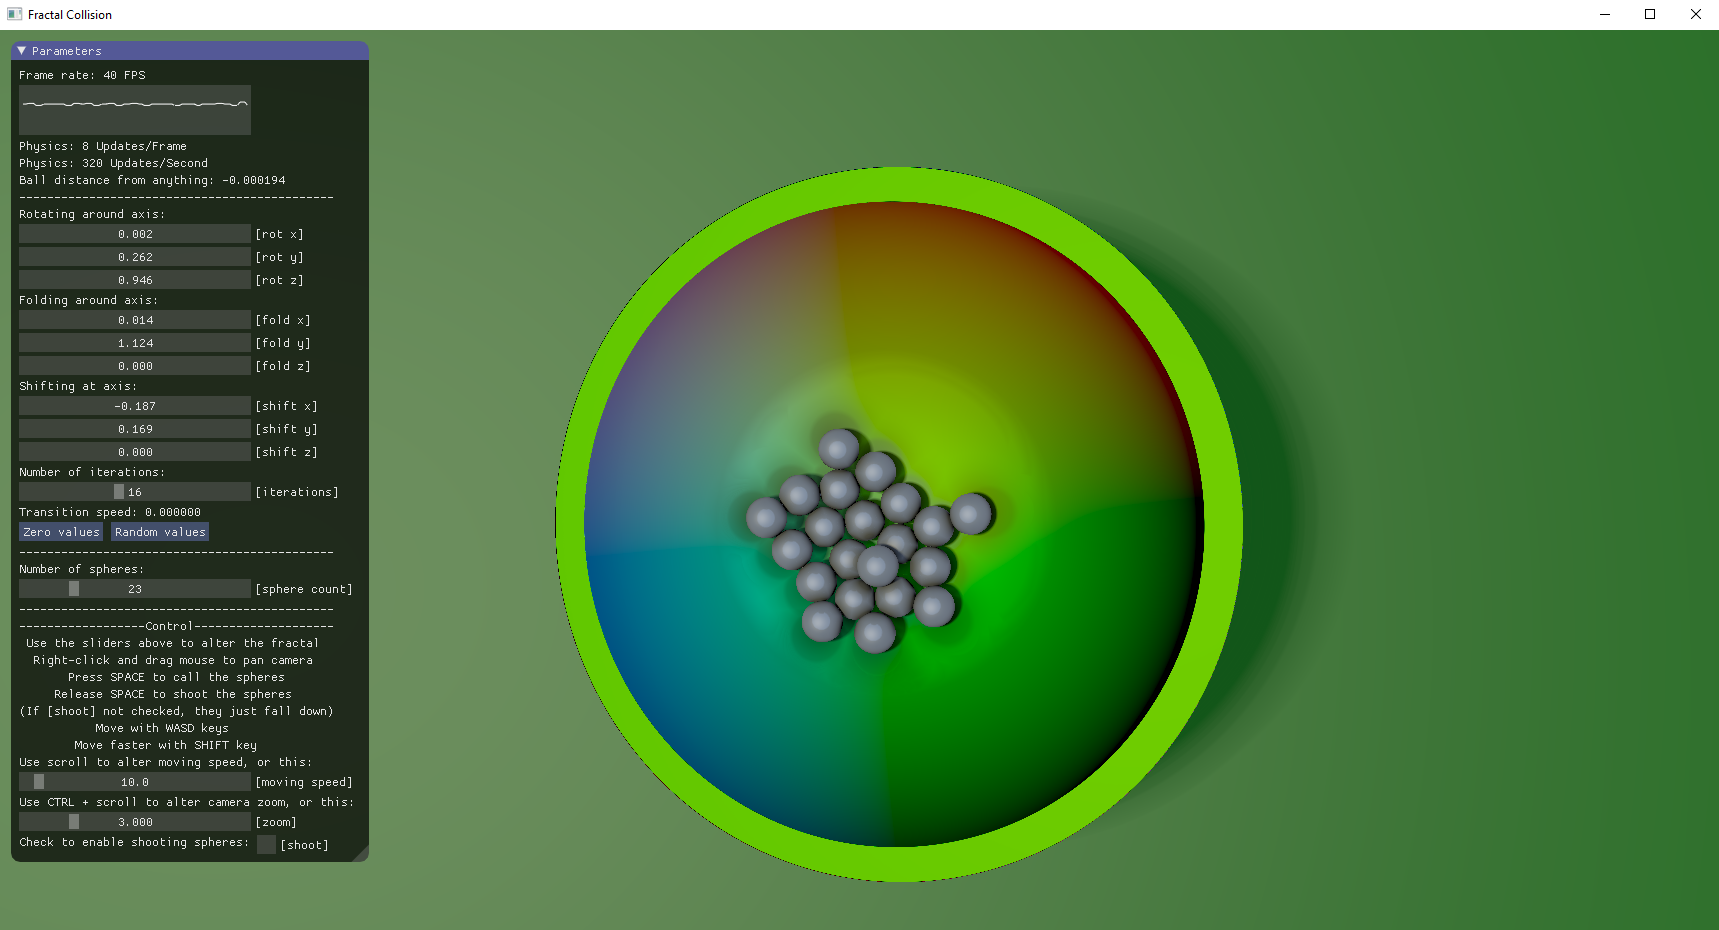
\includegraphics[width=0.7\textwidth, frame]{scrn2}
	\caption{A kiindulási pozíció alatt található alakzat néhány labdával}
	\label{fig:bowl}
\end{figure}

\cleardoublepage
\section{Megvalósítás}

A program írása során a Számítógépes Grafika BSc gyakorlat tárgy honlapjának \cite{GrafikaB26:online} projektjei nyújtottak kiindulási alapot. Az SDL működtetése és számos alapvető függvényhívás lett belőlük felhasználva.

\subsection{CMyApp osztály}

Ez a fő osztály. A \textbf{main.cpp} ezen keresztül kezeli le az egér és billentyűzet bemeneteit, szimulálja a fizikát és továbbítja a shaderbe a paramétereket hogy megtörténjen a kirajzolás. A fontosabb függvények külön részletezésre kerülnek.

\begin{figure}[H]
	\centering
	\subfigure[A diagram felső fele]{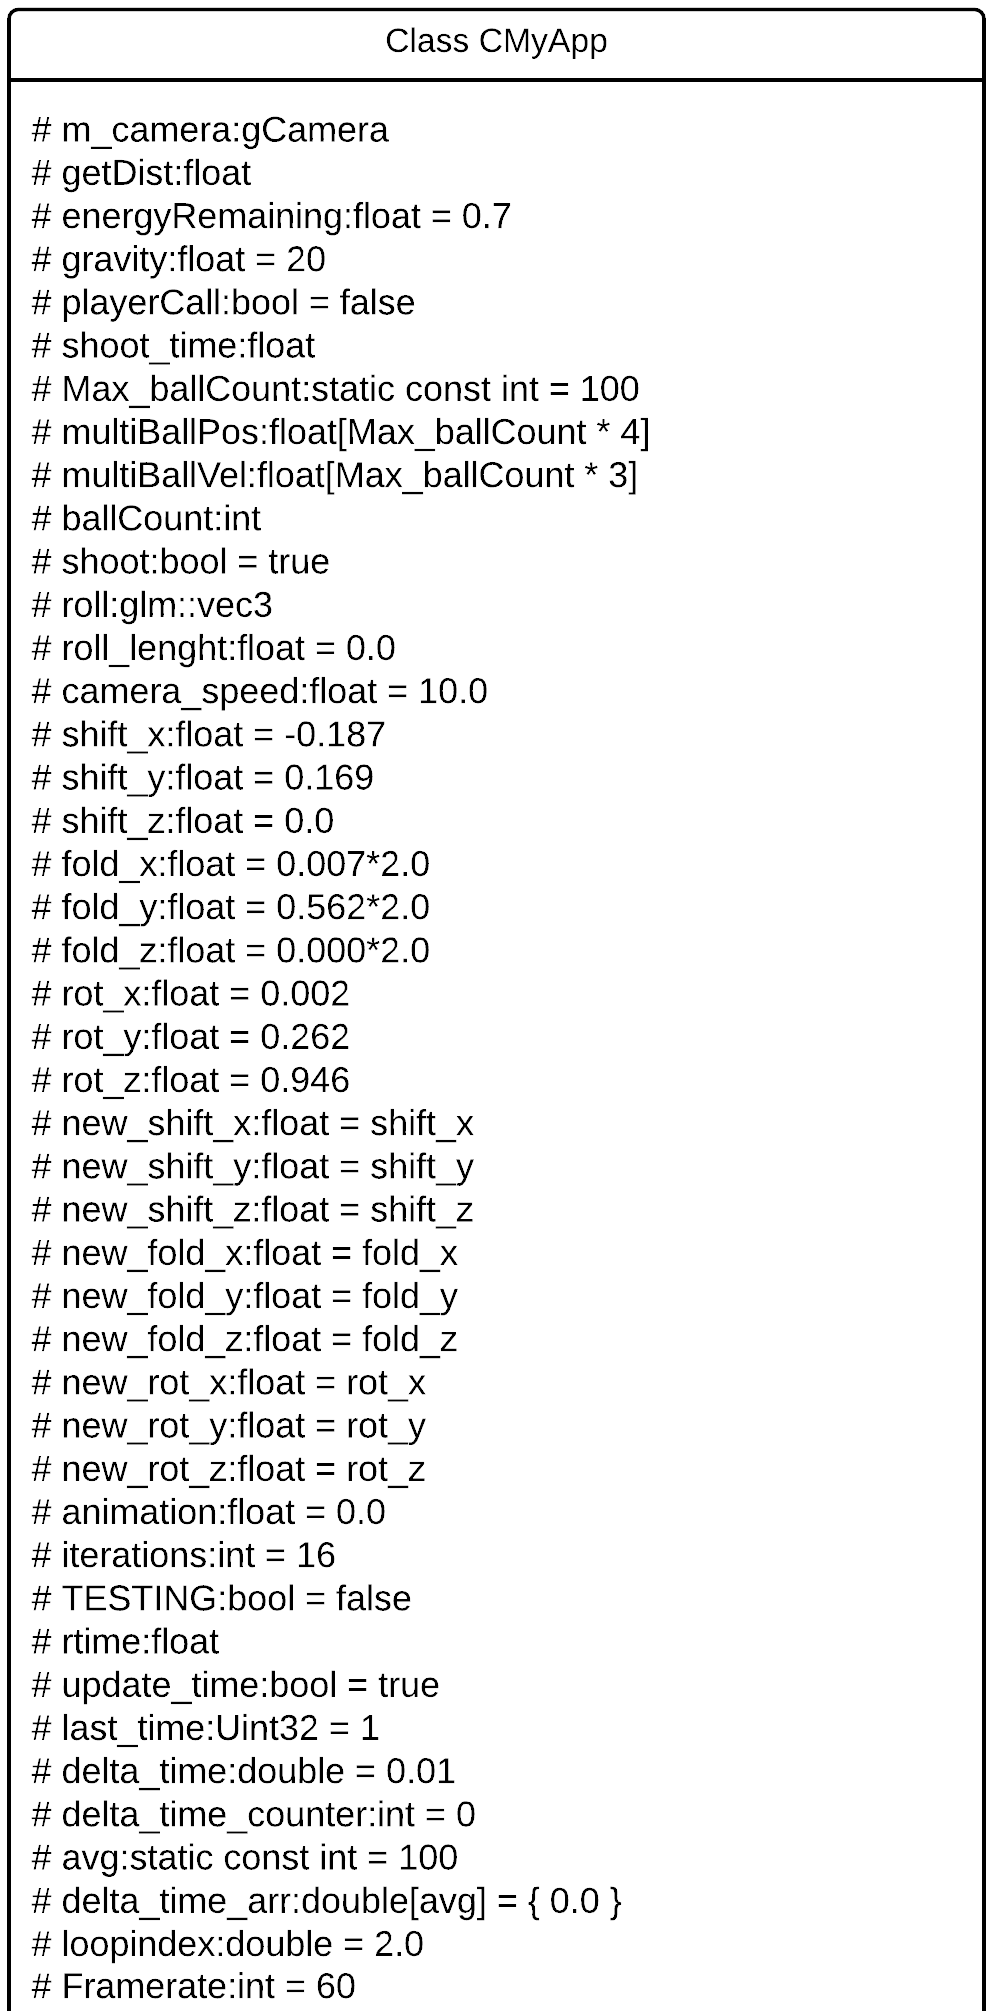
\includegraphics[width=0.4\linewidth]{cmyapp1}}
	\hspace{1pt}
	\subfigure[A diagram alsó fele]{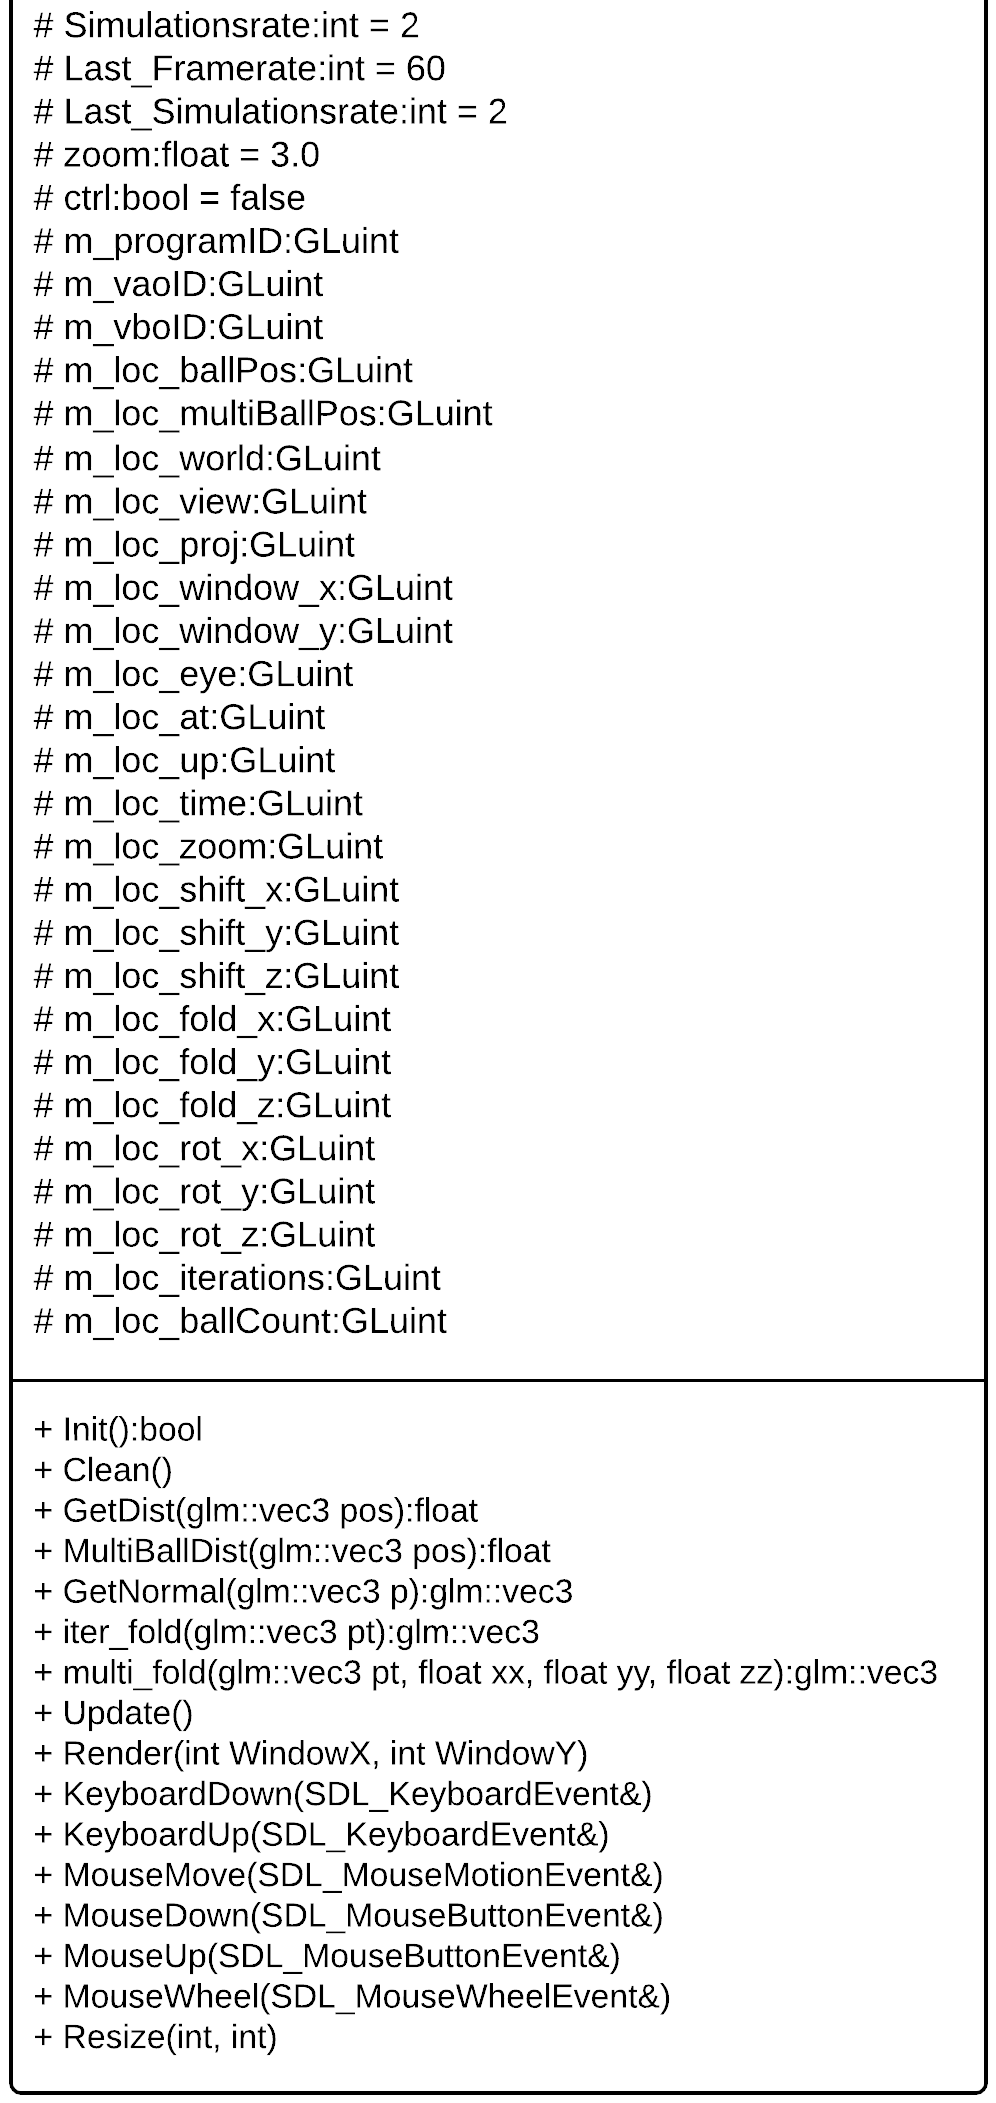
\includegraphics[width=0.4\linewidth]{cmyapp2}}
	\caption{A CMyApp osztálydiagramja (két részre szedve a hosszúsága miatt)}
	\label{fig:uml}
\end{figure}

\subsubsection{bool Init()}

Ebben inicializálódik minden aminek kell, itt foglaljuk le a grafikus erőforrásokat. Definiálunk két darab háromszöget melyek összerakva egy olyan négyzetlapot alkotnak ami az XY síkot (-1,-1)-től (1,1)-ig lefedik. Ez a négyzetlap lefedi a teljes ablakot és ennek a fragmanet shaderben való átszínezésével kapjuk meg a képet. Az uniform változók memóriacímeit és a shadereket is itt határozzuk meg, valamint a mozgatható labdák pozícióját, méretét és sebességét tartalmazó tömbök is itt kapnak kezdőértékeket.

\subsubsection{void Update()}

Minden képernyőfrissítés előtt lefut, ebben történik \textbf{az ütközések ellenőrzése} és a labdák mozgatása a pozícióik frissítése által. 

A labdák befogott pozíciói -- amikhez akkor közelítenek ha lenyomjuk a szóköz billentyűt -- itt kerülnek kiszámításra a kamerát leíró adatok ismeretében. Meg tudunk határozni egy a kamerából előre, egy jobbra és egy felfelé irányba mutató egységhosszú vektort. Ezek megfelelő kombinációjával és egy időtől és a labdák darabszámától függő forgatási mátrix felhasználásával tudjuk a pozíciójukat egy a kamerához képest fix helyzetű kör mentén beállítani. Mivel az időtől is függ a forgatási mátrix, így ezen kör mentén folyamatosan keringnek.

A labdák hívása és kilövése is itt van megvalósítva. A \textbf{SPACE} nyomva tartásakor a labdák az imént kiszámolt pozíciójának és a jelenlegi pozíciójának különbségének konstans-szorosát kapja meg sebességül. Ezáltal minél messzebb van a pozíciótól annál gyorsabban közeledik hozzá. Illetve csak a billentyű nyomva tartásakor frissül egy \textbf{shoot\_time} változóban az idő. 

Ha az aktuális idő és a \textbf{shoot\_time} közötti idő csak kis mértékben tér el akkor tudjuk hogy most lett felengedve a billentyű. Ekkor pedig a kamerából előrefelé mutató vektor konstans-szorosa adódik a labdák sebességéhez.

A labdák \textbf{ütközéseinek megállapításához} a kirajzoláshoz is használt távolságfüggvényt használjuk a vizsgált labda középpontjával. Ha ez a távolság kisebb mint a gömb sugara akkor tudjuk hogy valamivel ütköztünk.

A helyes \textbf{viselkedés megállapításához} ismerünk kell az ütközés pontjában a felületi normálist. A normális közelítő értékének kiszámolásához használt módszer (\ref{src:norm}. kódrészlet) a távolságfüggvényt használja, így egy egyszerűsítést tehetünk: az ütközési pont helyett a gömb középpontjában számoljuk a felületi normálist! Ezáltal az éleken és sarkokon, ahol felületi normális nem igazán értelmezhető, ott is jó viselkedést produkáló vektort fogjuk kapni.

\lstset{caption={A felületi normálist kiszámoló függvény}, label=src:norm}
\begin{lstlisting}[language={C++}]
glm::vec3 CMyApp::GetNormal(glm::vec3 p) {
	float d = GetDist(p);
	float e = 0.0005;
	glm::vec3 n = d - glm::vec3(
		GetDist(p - glm::vec3(e, 0, 0)),
		GetDist(p - glm::vec3(0, e, 0)),
		GetDist(p - glm::vec3(0, 0, e)));
	return glm::normalize(n);
}}
\end{lstlisting}

Ezután már csak a kapott normális által meghatározott síkra kell visszavernünk\footnote{Ez a normálisra való tengelyes tükrözést és egy $-1$-el való szorzást jelent} a vizsgált labdánk sebességvektorát és a megfelelő komponenseit némileg csökkenteni, ezzel szimulálva hogy visszapattanáskor veszít egy keveset az energiájából -- ehhez is a normálist használhatjuk, azért kell komponensenként mert a valóságban ha például elrúgunk ívesen egy focilabdát, akkor annak az vízszintes irányú mozgási energiája jóval kevesebbet csökken visszapattanáskor mint a függőleges irányú -- a mozgási energia egy része ugyanis perdületivé alakul.

Fel kell arra is készülnünk ha a \textbf{labdánk belemegy egy másik objektumba}. Ez többnyire akkor történik meg ha nagyon gyorsan mozog a labda és két ellenőrzés között beleér, vagy ha a labda tartásakor direkt belevisszük egy objektumba. Ha benne vagyunk valamiben akkor frissítjük a pozíció értékét a normális irányába egy kis mértékben. Ezáltal ha esetleg belekerülne valamibe a labdánk akkor kijön belőle automatikusan.

\begin{figure}[H]
	\centering
	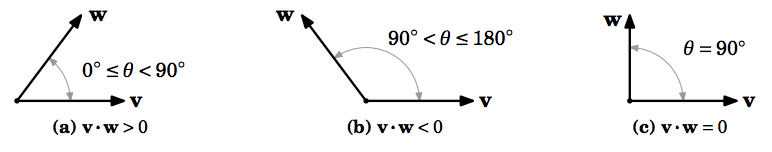
\includegraphics[width=0.8\textwidth]{dot}
	\caption{A skaláris szorzat előjele és a vektorok közötti szög összefüggése \cite{13DotPro51:online}}
	\label{fig:dot}
\end{figure}

Mivel tudjuk hogy akár egy másik objektumba is belemehet a labdánk ezért még egy esetre fel kell készülnünk: a másik objektumból kifelé jövet nem szeretnénk hogy ismét tükröződjön a sebességvektor, hiszen akkor állandóan oda-vissza tükröződne és sosem jutna ki a labda. Erre megoldás hogy csak akkor tükrözzük a sebességvektort ha a normálvektorral bezárt szöge \textbf{tompaszög}. Ehhez mindössze a két vektor skaláris szorzatát kell venni és ellenőrizni hogy az eredmény negatív-e. (\ref{fig:dot}. ábra)

 
\subsubsection{void Render(int WindowX, int WindowY)} 

Paraméterként megkapja az ablak méreteit. Az imgui panel ebben a függvényben hívódik meg és töltődik fel a megjelenített tartalommal, illetve itt kapják meg a felületen bevitt értékeket a megfelelő változók. Itt hívódik meg továbba a shader is, melynek rengeteg uniform válozót adunk át:
\begin{compactitem}
	\item \textbf{WindowX, WindowY} -- az ablak méretei
	\item \textbf{eye, at, up} -- a kamerát definiáló vektorok
	\item \textbf{rtime} -- az indítás óta eltelt idő másodpercben
	\item \textbf{multiBallPos} -- a mozgó labdák koordinátáit és méreteit tartalmazó tömb
	\item \textbf{shift\_x, shift\_y, shift\_z} -- az eltolás transzfomácó paraméterei
	\item \textbf{fold\_x, fold\_y, fold\_z} -- a tükrözés tranformációk paraméterei
	\item \textbf{rot\_x, rot\_y, rot\_z} -- a forgatás traszformáció paraméterei
	\item \textbf{iterations} -- a fraktál iterációinak száma
	\item \textbf{ballCount} -- a mozgó labdák száma
	\item \textbf{zoom} -- a kamera látószögét befolyásoló paraméter
\end{compactitem}

A kép megalkotása teljes egészében a shaderben történik. Miután megtörtént az imgui panel konfigurásála és az uniform változók átadása, a \textbf{glDrawArrays()} függvény hívásával a vertex shaderbe juttatjuk az inicializáció során létrehozott és a futás során sehol nem módosított négyzetet.

A megadott négyzetünk a várt koordináták miatt (\ref{fig:NDC}. ábra) lefedi a teljes ablakot, viszont ha az ablak nem négyzet alakú, akkor torzítás történik. A vertex shaderben az ablak méreteinek ismeretében kompenzáljuk a torzítást, azáltal hogy a továbbadott vektor x komponensét megszorozzuk az ablak szélességének és magasságának hányadosával. 

\begin{figure}[H]
	\centering
	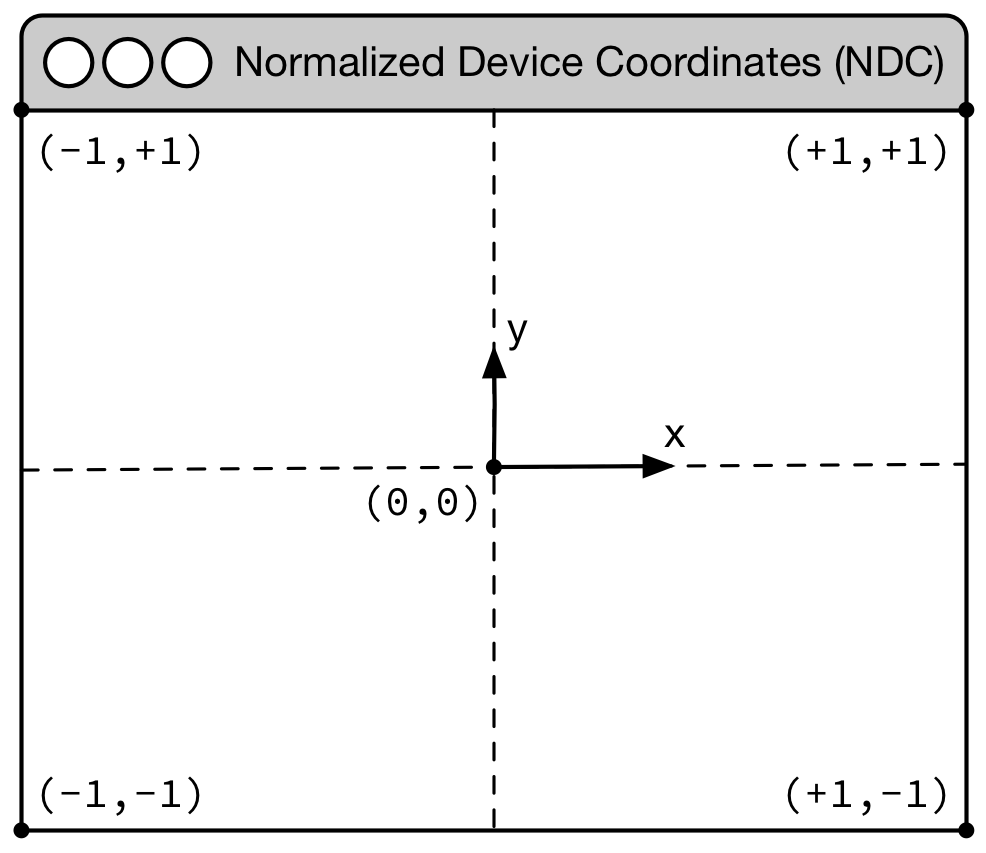
\includegraphics[width=0.6\textwidth]{NDC}
	\caption{NDC (Normalized Device Coordinates) - az ablak koordinátái \cite{PythonOp51:online} }
	\label{fig:NDC}
\end{figure}

Ennek köszönhetően a fragment shaderben a bemeneti vektorunk már torzításmentesen reprezentálja az ablakunk koordinátáit. Ezután a fragment shaderben \aref{sec:kepmod}. fejezetben ismertetett elmélet alapján megalkotársa kerül a kép.

\subsection{gCamera osztály}

Ez az osztály egy általános megvalósítása egy virtuális kamerának és közel egy-az egyben lett felhasználva a Számítógépes Grafika BSc gyakorlat tárgy honlapjának \cite{GrafikaB26:online} projektjeiből. 

Csak a kamerát mozgató függvényekre és az általuk befolyásolt eye, at és up vektorokra van szükség. Ezen három vektor segítségével lehet majd a shaderben megállapítani a sugarak irányát és kiindulási pontját.

\begin{figure}[H]
	\centering
	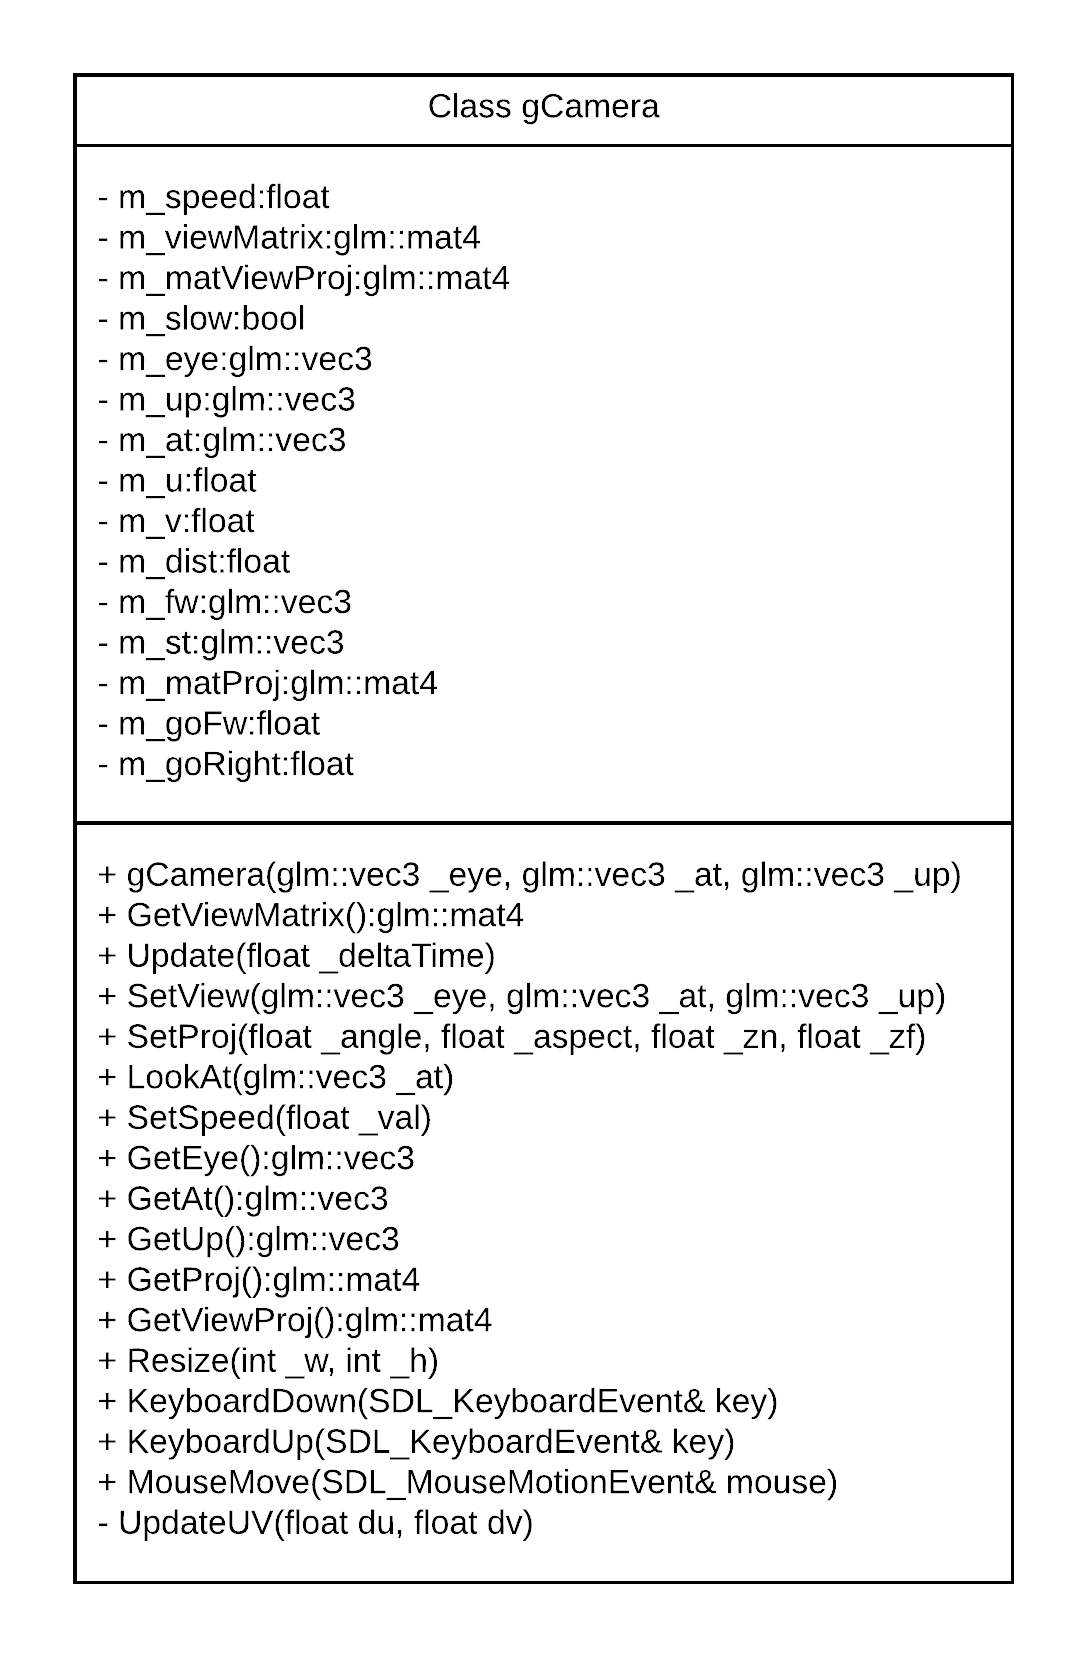
\includegraphics[width=0.6\textwidth]{gcam}
	\caption{A gCamera osztálydiagrammja}
	\label{fig:gcam}
\end{figure}

Ebben az osztályban valósul meg a virtuális kamera mozgatása, hiszen a helyváltoztatáshoz mindössze a kamerát leíró vektorokat kell megfelelően transzfomálni. Az ehhez szükséges függvények kerülnek részletezésre.

\subsubsection{void Update(float \_deltaTime)}

Ez a függvény minden kirajzolás előtt meghívódik és frissíti a kamerát definiáló vektorokat. Ehhez ismernünk kell az előre (\textbf{m\_fw}) és az oldalra mutató (\textbf{m\_st}) vektorokat, melyeket a megfelelő szorzóval egyszerűen hozzáadunk az \textbf{eye} és \textbf{at} pozícióvektorainkhoz (\textbf{m\_eye} és \textbf{m\_at}) ahogyan azt \aref{src:updt}. kódrészletben is láthatjuk.

\lstset{caption={Az \textbf{eye} és \textbf{at} vektorok frissítése}, label=src:updt}
\begin{lstlisting}[language={C++}]
	m_eye += (m_goFw*m_fw + m_goRight*m_st)*m_speed*_deltaTime;
	m_at  += (m_goFw*m_fw + m_goRight*m_st)*m_speed*_deltaTime;
\end{lstlisting}

A szorzókat (\textbf{m\_goFw} és \textbf{m\_goRight}) a billenytűk fogják szabályozni. Megfigyelhetjük ha ezen változók értéke $+1$ vagy $-1$ akkor előre-hátra és jobbra-ballra is tudunk menni. Ellenben ha mindkettő nulla, akkor nem változnak az \textbf{eye} és \textbf{at} vektoriank, vagyis ekkor nem fog mozogni a virtuális kamera. 

Látható továbbá hogy a mozgás mértéke az \textbf{m\_speed} változótól és a \textbf{\_deltaTime-tól} fognak függeni. A felületen az \textbf{m\_speed} értékét állítjuk át az osztály \textbf{SetSpeed(float \_val)} függvényen keresztül, ezzel szabályozván a mozgási sebességet.


\subsubsection{void KeyboardDown(SDL\_KeyboardEvent\& key) }

A \textbf{WASD} és a \textbf{SHIFT} billentyűk segítségével tudunk mozogni a térben ezért ezeket a billenytűket folyamatason figyelni kell hogy le vannak-e nyomva. Ez egy switch és a paraméterül kapott esemény segítségével történik meg.

A \textbf{W} és \textbf{S} billentyűk lenyomására az \textbf{m\_goFw} változó értéke rendre $+1$ és $-1$ értéket kap. Az \textbf{A} és \textbf{D} billentyűk hatására pedig hasonlóképpen az \textbf{m\_goRight} változónak adunk $+1$ és $-1$ értéket.

A \textbf{SHIFT} billentyű lenyomására, ha az \textbf{m\_slow} változó értéke hamis, akkor az \textbf{m\_speed} változó értékét növeljük a négyszeresére, illetve az \textbf{m\_slow-t} igazra állítjuk. Azért szükséges ezen változó figyelése mert csak egyszer szeretnénk megnégyszerezni a sebességet. 

\subsubsection{void KeyboardUp(SDL\_KeyboardEvent\& key) }

A billentyűk felengedését külön kell kezelni, ez ugyanolyan elven történik mint a \textbf{KeyboardDown()} esetében: A \textbf{W} és \textbf{S} billentyűk felengedésére az \textbf{m\_goFw} változó értéke 0 lesz. Az \textbf{A} és \textbf{D} billentyűk felengedésére pedig az \textbf{m\_goRight} változót nullázzuk.

A \textbf{SHIFT} billentyű felengedésére, ha az \textbf{m\_slow} változó éréke igaz, akkor az \textbf{m\_speed} változó értékét változtatjuk a negyedére, valamint az \textbf{m\_slow} hamis lesz.

\subsubsection{void UpdateUV(float du, float dv)}

Ez a függvény \aref{src:updt}. kódrészletben is látható \textbf{m\_fw} és \textbf{m\_st}, vagyis az előre és oladra mutató vektoroknak fog megfelelő értéket adni és frissíti az \textbf{m\_at} vektorunkat. Az osztály \textbf{MouseMove(SDL\_MouseMotionEvent\& mouse)} függvénye fogja megadni neki a \textbf{du} és \textbf{dv} paramétereket az egér függőleges és vízszintes elmozdulása alapján. Ez is minden kirajzolás előtt meghívódik.

\begin{figure}[H]
	\centering
	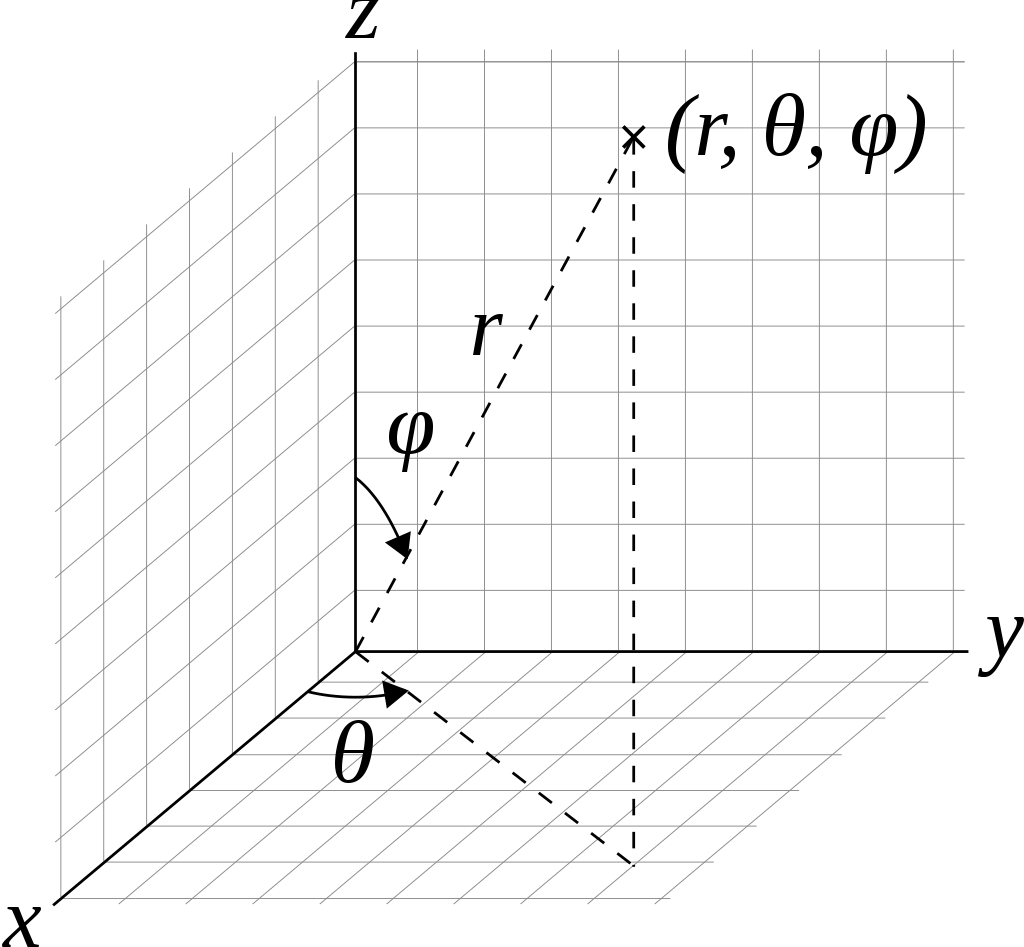
\includegraphics[width=0.5\textwidth]{polar}
	\caption{Polár koordinták \cite{Spherica72:online}}
	\label{fig:polar}
\end{figure}

Az \textbf{m\_at} vektorunkat (mely azt határozza meg hogy merre néz a kamera) leírjuk polárkoordinátákkal és a megfelelő szögekhez hozzáadjuk -- az értelmezési tarttományok figyelembe vételével -- a paraméterül kapott \textbf{du} és \textbf{dv} értékeket. Ezután átszámoljuk az így kapott vektort Descartes-féle koordinátákra és ez lesz a \textbf{m\_at} vektorunk új értéke.

Az \textbf{m\_fw} vetort az \textbf{m\_at} és \textbf{m\_eye} különbsége fogja adni, az \textbf{m\_st} vetort pedig a \textbf{m\_fw} és \textbf{m\_up} vektoriális szorzata.

\subsection{Fragment shader}
A megjelenítés lényegi munkáját a fragment shader végzi, \aref{sec:kepmod}. alfejezetben a képalkotás elméleti része már nagy vonalakban ismertetve lett, ebben az alfejezetben ennek az implementációját mutatom be. A függvények ismertetésének sorrendje nagyságrendileg a meghívásuk sorrendjét követi.

\subsubsection{void main()}
Az unifom változóként megkapott \textbf{eye, at} és \textbf{up} vektorok és a vertex shaderből érkező normalizált ablakkoordináták segítségével, valamint néhány vektorművelet felhasználásval kiszámoljuk a sugarak kiinduló pontját és irányát. Ezt átadjuk a \textbf{render()} függvénynek ami visszatér az adott pixel színével.

\subsubsection{vec3 render(vec3 ro, vec3 rd)}
A paramétereivel meghívja a \textbf{RayMarch()} függvényt, mellyel meg tudjuk határozni hogy az aktuális sugár a virtuális terünk mely pontjában ütközött. Ebben a pontban a \textbf{GetNormal()} függvénnyel meghatározzuk a felületi normálist. Ezek ismeretében az alkalmazott fénymodellünkkel\footnote{\Aref{sec:lighting}. fejezetben a fénymodellről már volt szó, az implementációját nagyon hosszan lehetne részletezni de többnyire szabány megoldások és önmagyarázó kódokal készült, így erre nem kerül sor.} meg tudjuk állapítni hogy milyen színű legyen a paraméterként megkapott sugárnyalábhoz tartozó pixelünk és ennek az rgb kódjával tér vissza a függvény. 

\subsubsection{vec3 GetNormal(vec3 p)}
A paraméterként kapott pontban kiszámolja a felületi normális egy közelítését. Ezt meghatározzuk a differenciaképlet (\ref{eq:normal}. képlet) alapján az adott pontban és az eredményt normálizáljuk. Az \textbf{$\epsilon$} értékét az implementációban 0.001-nek választottam. Ha az érték túl nagy, akkor pontatlan lesz a közelítés, ha túl kicsi akkor pedig a számábrázolás pontatlansága okozhatja a kapott nomra pontatlanságát.
\begin{equation}
\label{eq:normal}
f^{\prime}(x, y, z)\approx\frac{1}{\epsilon} \cdot\left[\begin{array}{l}
f(x, y, z)-f(x-\epsilon, y, z) \\
f(x, y, z)-f(x, y-\epsilon, z) \\
f(x, y, z)-f(x, y, z-\epsilon)
\end{array}\right]
\end{equation}



\subsubsection{float RayMarch(vec3 ro, vec3 rd)}
\Aref{sec:kepmod}. fejezetben az algoritmus implementációja és leírása is érintve lett. Meghívódik benne a \textbf{GetDist()} névvel illetetett távolságfüggvény. A felületi távolsággal kapcsolatos kilépési feltétel javításán kívül ez egy szabvány implementációja a \textbf{Sphere tracing} algoritmusnak.

\subsubsection{float GetDist(vec3 pos, out float col)}
A paraméterül kapott \textbf{pos} ponttól kiszámolja az összes felület uniójától vett távolságot. A testek felületét leíró függvények Ingio Quilez honlapján \cite{InigoQui87:online} található gyűjteményből származnak. Összességében a sík, a téglatest és a gömb függvényei vannak különféle módon tarszformálva. Minden alakzathoz tarozó függvény visszatér a megfelelő távolsággal, majd ezeknek a minimuma lesz a függvény visszatérési értéke. 

A függvénynek van egy out paramétere is, amit nem kell feltétlenül megadnunk. Ez a paraméter annak függvényében kap értéket hogy melyik objektumtól származik a legkisebb távolságérték. Ez az érték akkor kerül ellenőrzésre a \textbf{render()}-ben amikor a \textbf{RayMarch()} segítségével már megállípatottuk hogy hol állt meg a kiküldött sugárnyaláb. Ezen érték felhasználásával minden objektumnak adhatunk egy a fényektől és megvilágítsától független alapszínt.

Ez az alapszín egyébként a fraktál esetén a felületi normális átkonvertálva rgb értékekbe. Ugyanezt a színezési technikát kapja a a kezdeti pozíció alatt található félgömbhéj is. 

A fraktálunk pedig egy egyszerű téglatest amire az \textbf{iter\_fold()} transzofmációs függvény lett alkalmazva.

\subsubsection{vec3 iter\_fold(vec3 pt)}
Paraméterül egy pontot kap, amire az adott traszformációkat elvégzi, majd a transzformált ponttal tér vissza. Ez a függvény egy ciklust tartalmaz, mely az unifom változóként megkaptt \textbf{iterations}-szor fogja megismételni minden tengelyre az eltolás, forgatás és fold traszformációkat -- amiket unifom változóként megkapott paraméterekkel hajt végre -- egymás után a kapott pontra.

\begin{description}
	\item[Az eltolás] pont esetében csak annyit tesz hogy a megfelelő koordiátákból kivonjuk az eltolás koordinátáit.
	\item[A forgatás] a klasszikus 3 dimenziós forgatási mátrixokra épül:
$$\begin{array}{l}
R_{x, \vartheta}=\left[\begin{array}{ccc}
1 & 0 & 0 \\
0 & \cos (\vartheta) & -\sin (\vartheta) \\
0 & \sin (\vartheta) & \cos (\vartheta)
\end{array}\right] \\
\\
R_{y, \vartheta}=\left[\begin{array}{ccc}
\cos (\vartheta) & 0 & \sin (\vartheta) \\
0 & 1 & 0 \\
-\sin (\vartheta) & 0 & \cos (\vartheta)
\end{array}\right] \\
\\
R_{z, \vartheta}=\left[\begin{array}{ccc}
\cos (\vartheta) & -\sin (\vartheta) & 0 \\
\sin (\vartheta) & \cos (\vartheta) & 0 \\
0 & 0 & 1
\end{array}\right]
\end{array}$$
	\item[Fold] (kvázi tükrözés) egy eltolás a megadott síkra merőlegesen, úgy hogy annyival kerül eltolásra amilyen távolságra van a megadott síktól. Csak a sík egyik oldalán lévő pontokkal végezzül el ezt, a másik oldalán lévő pontokat nem mozdítjuk. Ezáltal már nem lesz egybevágósági traszformáció, és emiatt nem is mondható tükrözésnek, ezért lett a \textbf{fold} kifejezés használva rá.
\end{description}

Fontos hogy a transzformációk között legyen olyan ami nem egybevágósági transzformáció, amennyiben nem lenne akkor hiába iterálnánk akármennyit, az alakzat formája nem változna. Lényegében ez az egyetlen kikötése a fraktál generátornak, amíg ez teljesül addig tetszőlegesen variálhatjuk a traszformációkat hogy hatékonyabban lehessen kiszámolni az alakzatot, vagy éppen izgalmasabb formákat kapjunk.

\section{Tesztelés}

A tesztelés során megvizsgáltam hogy a funkciók (\ref{sec:ui}.~fejezet) az elvártaknak megfelelően működne-e. Az ehhez használt számítógép konfiguráció:
\begin{compactitem}
	\item Intel® Core™ i7-8700 CPU
	\item 16 GB RAM
	\item NVIDIA GeForce GTX 1660 GPU
	\item Windows 10 operációs rendszer
\end{compactitem}

\cleardoublepage
\subsection{Működés helyessége}

A következő viselkedéseket ellenőriztem:
\begin{compactenum}
	\item A virtuális kamerát lehet forgatni az \textbf{egérrel};
	\item A virtuális kamera nagyítását lehet állítani a \textbf{CTRL + görgővel} és a csúszkával is;
	\item A virtuális kamerát lehet mozgatni a \textbf{WASD} billentyűkkel;
	\item A mozgás sebességét lehet gyorsítani a \textbf{SHIFT} billentyűvel és állítani a görgővel vagy a csúszkával;
	\item Ha egyszerre gyorsítunk \textbf{SHIFT}-tel és görgővel, a görgő sebessége felülírja a shift gyorsítását;
	\item A fraktál paramétereit át lehet állítani a \textbf{csúszkákkal} és a fraktál ezen értékeknek megfelelően változik;
	\begin{figure}[H]
	\centering
	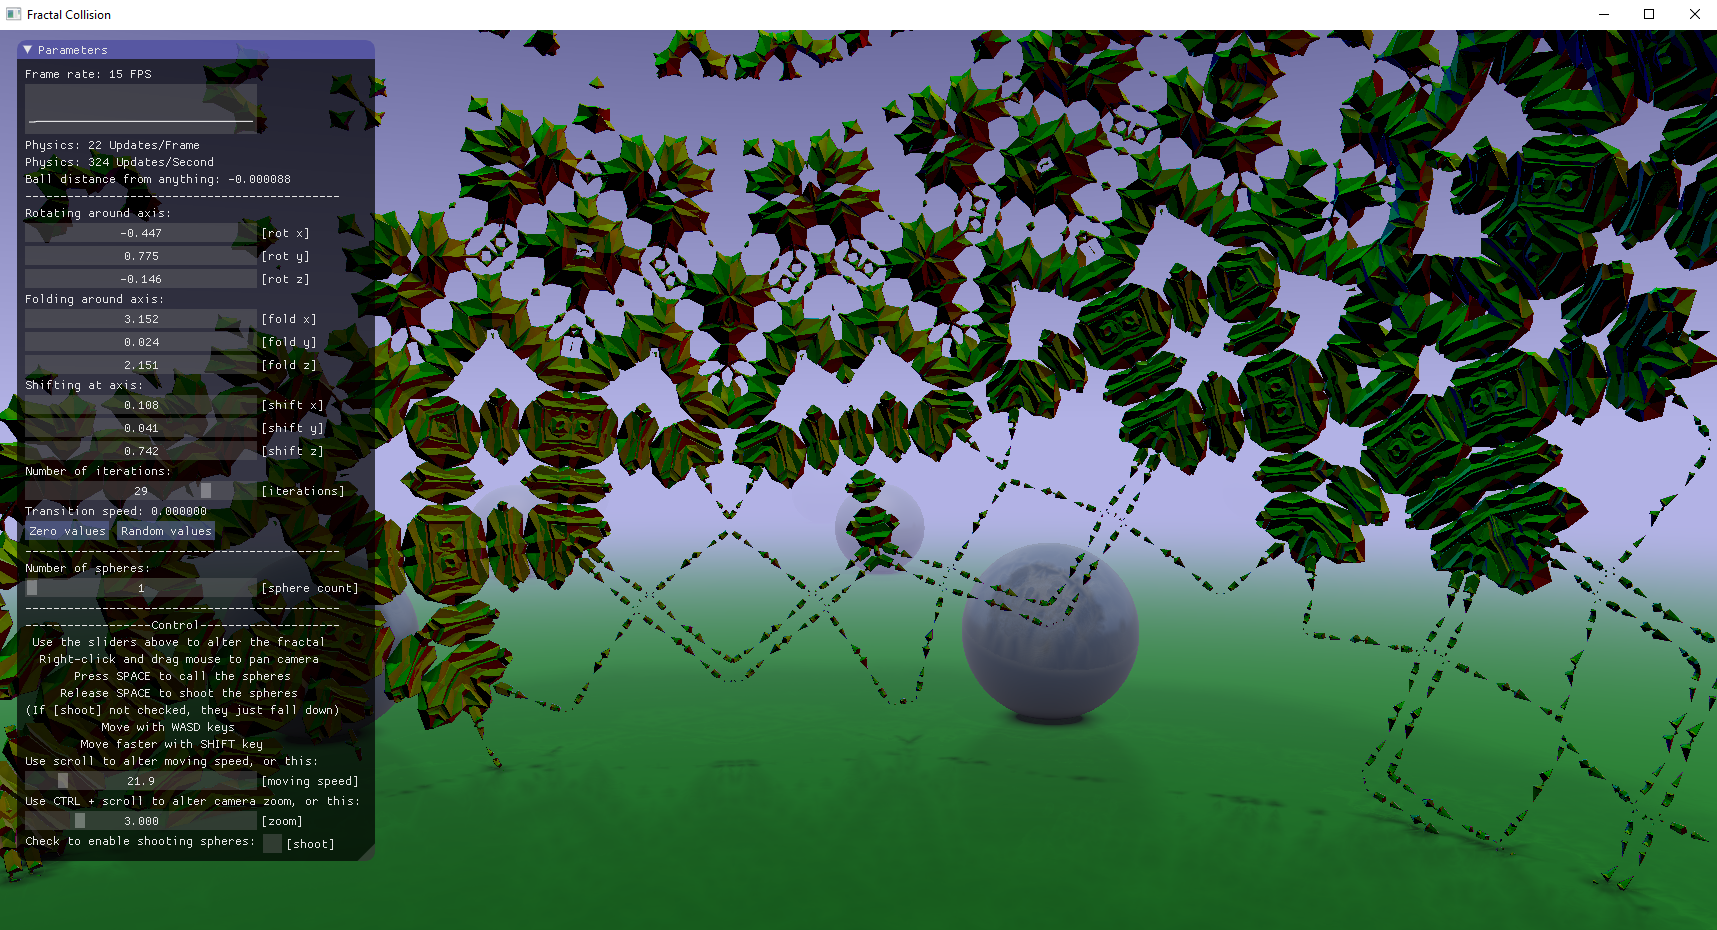
\includegraphics[width=0.9\textwidth,frame]{scrn7}
	\caption{A paraméterek egy lehetséges kombinációja amikor már éppen csak látható a fraktál, kicsit módosítva a megfelelőkön már nem látható}
	\label{fig:extr}
    \end{figure}
	\item A \textbf{``Zero values''} gomb hatására megközelíti minden érték a nullát;
	\item A \textbf{``Zero values''} gomb extrém érték esetén: 10000-re állítva egy csúszkát "nullázás" után az értéke 0.481 lett, 36-os iteráció mellett;
	\item A \textbf{``Random values''} gomb valóban véletlenszerű értékeket állít be. Időnként nem látható fraktálokat eredményez (\ref{fig:extr}. ábra), minél nagyobb az iterácó értéke annál gyakrabban;
	\item A \textbf{SPACE} billentyű nyomva tartásakor a labdák megjelennek a felhasználó előtt. Ha közeli akadályba ütköztek akkor nem tudnak;
	\item A \textbf{SPACE} billentyű felengedésekor a labdák kilövődnek ha be van pipálva a \textbf{[shoot]}, és leesnek a gravitációnak megfelelően ha nincsen;
\begin{figure}[H]
	\centering
	\subfigure[Nagyon sok labda]{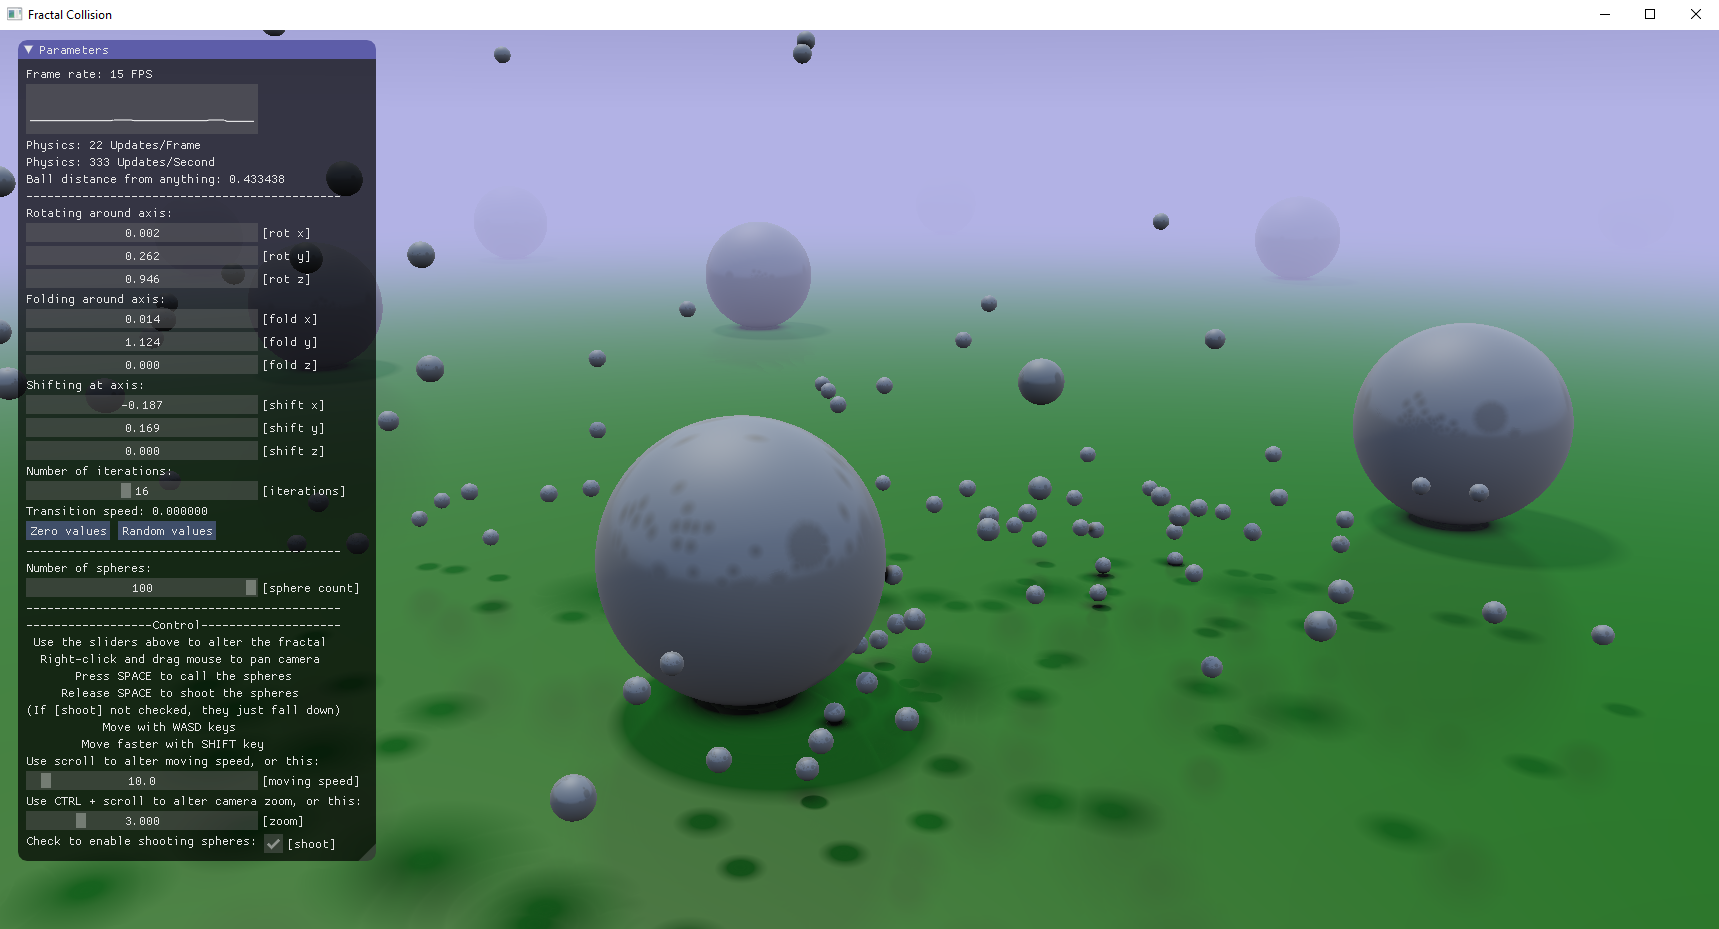
\includegraphics[width=0.7\linewidth, frame]{scrn8}}
	\hspace{1pt}
	\subfigure[Extrém fraktál]{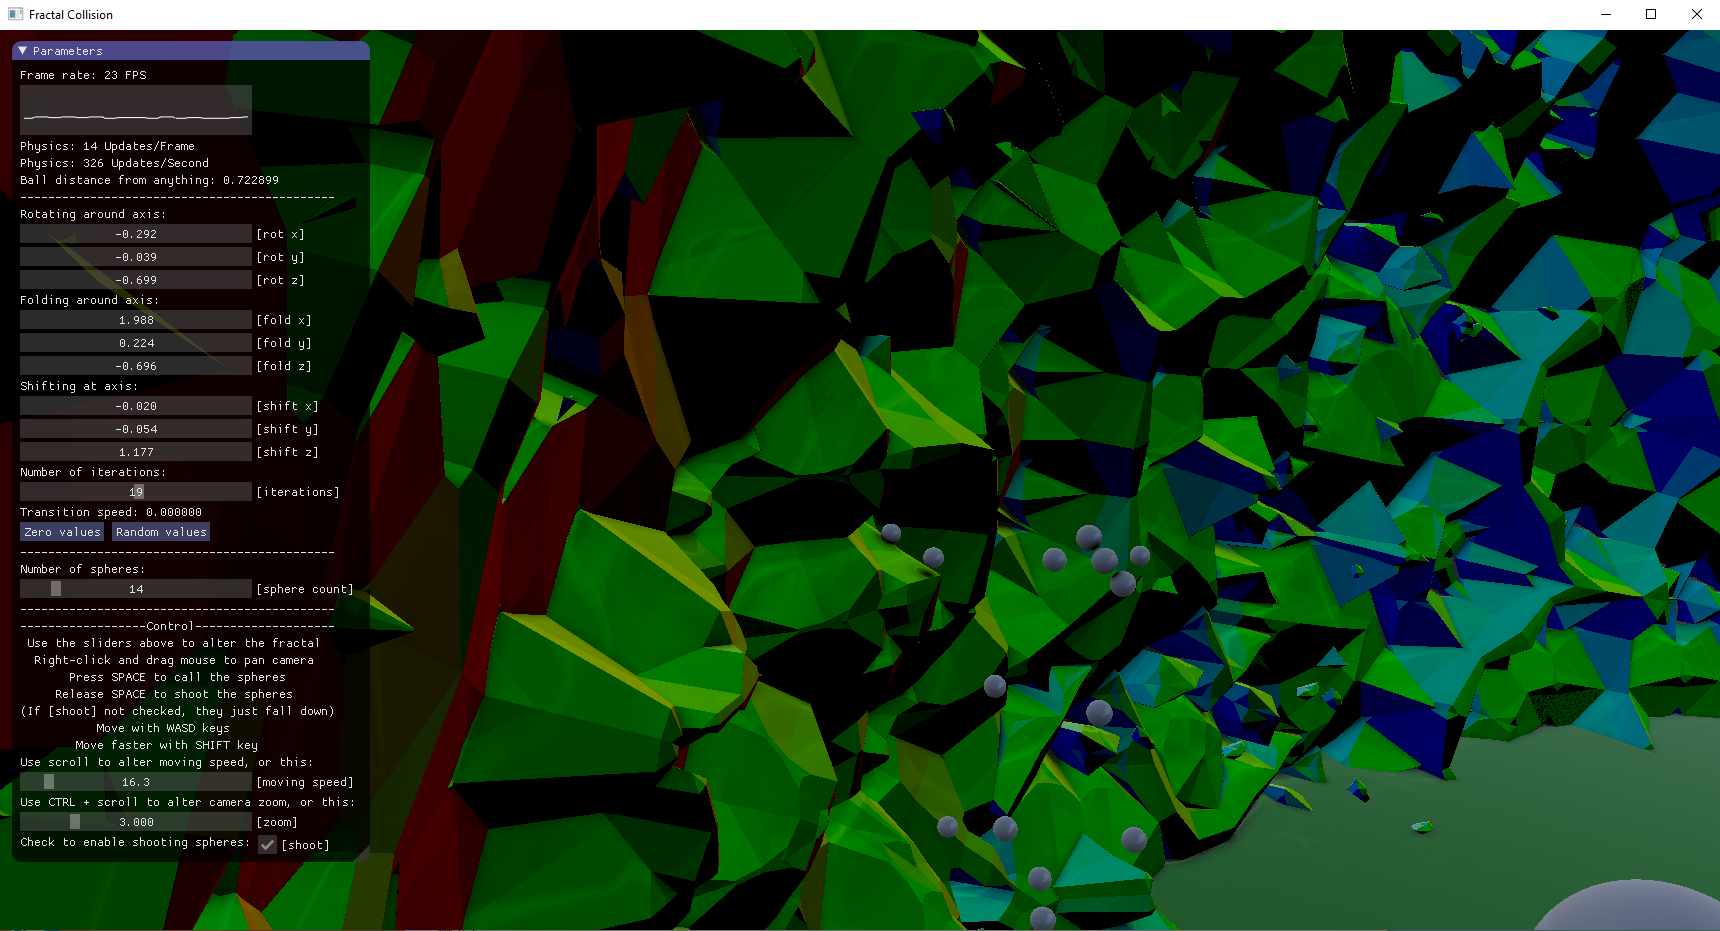
\includegraphics[width=0.7\linewidth, frame]{scrn3}}
	\caption{A labdák ütközése különböző körülmények között}
	\label{fig:hit}
\end{figure}
	\item A \textbf{labdák} ütközése tárgyakkal valósághűnek tűnik (\ref{fig:hit}. ábra);
	\item A \textbf{labdák} ütközése egymással közepesen valóságosnak tűnik, a kezdőpozíció alatti félgömbhéjban folyamatosan eltolják egymást.
	\item A \textbf{labdák} legurulása lejtős felületeken lassabb mint kellene, közepesen valósághű.
	\item A \textbf{labdák} legurulása lejtős felületeken nem egyenletes, bizonyos irányú lejtők kevésbé működnek jól.
\end{compactenum}


\cleardoublepage
\subsection{Teljesítmény}

Az alkalmazás erősen GPU igényes.  A futás teljesítményét az alábbi kód segítségével teszteltem:
\lstset{caption={A tesztelést végző kód}, label=src:test}
\begin{lstlisting}[language={C++}]
if (TESTING)
	{
		if (delta_time_counter < avg)
		{
			delta_time_arr[delta_time_counter] = delta_time;
			++delta_time_counter;
		}
		else
		{
			delta_time_counter = 0;
			double avg_delta_time = 0.0;
			for (int i = 0; i < avg; ++i) { avg_delta_time += delta_time_arr[i]; }
			avg_delta_time /= avg;
			printf("Avrage of delta time: %f ms   Iterations: %d   Number of spheres: %d \n", avg_delta_time*1000, iterations, ballCount);
			iterations += 2;
		}
	}
\end{lstlisting}

A kód az \textbf{Update()} függvény alján található. A \textbf{delta\_time} két képfrissítés között eltelt időt jelöli. Ezen kód segítségével \textbf{avg} darab képfrissítési idő átlagát vesszük, ezt kiírjuk az aktuális iterációk száma és mozgatható gömbök száma mellett a terminálablakra, majd ez előbbi értékét megnöveljük kettővel. A tesztek $avg=100$ értékkel futottak.

A tesztelés idejére ki lett kapcsolva a \textbf{vsync}, hogy ne befolyásolja a mérést. Ha be lenne kapcsolva akkor az $1/60 s = 16.66 ms$-nál kisebb kirajzolási idők eredményét nem tudnánk lemérni. Továbbá az a funkció is ideiglenesen ki lett kapcsolva ami alacsony képfrissítési ráta mellett kisebbre veszi az iterációk és gömbök számát.

A kezdeti pozícióhoz képest a kamera nem volt megmozdítva, valamint a tesztben érintett két paraméteren felül más nem lett átállítva a kezdeti alapértelmezettekhez képest. A futás eredményéből készült grafikon \aref{fig:Test1}.~ábrán látható.

\begin{figure}[H]
	\centering
	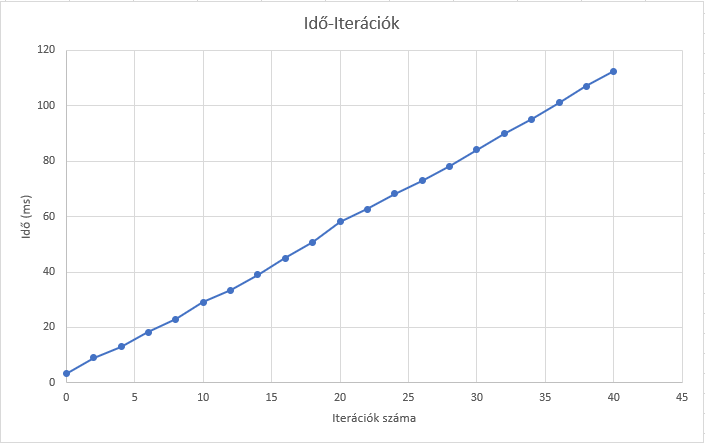
\includegraphics[width=0.8\textwidth,frame]{Test1b}
	\caption{Teljesítményteszt az iterációk számának függvényében}
	\label{fig:Test1}
\end{figure}


Megfigyelhető \aref{fig:Test1}. ábrán hogy az iterációk számától lineárisan függ a képfrissítési idő. Az adatok alapján az iterációk számának eggyel való növelése átlagosan nagyjából 2.8 ms-os növekedést okoz a renderelési időben a teszteléshez használt konfiguráción. Ebből adódóan nem érdemes nagyon magas iterációs számmal dolgozni, mert hamar szaggatott lehet a kirajzolás.

Ha \aref{src:test}.~kód 15. sorát átírjuk \textbf{ballCount += 5} -re akkor azt is meg tudjuk vizsgálni hogy az mozgatható gömbök (labdák) száma hogyan hat a képfrissítési időre. Ezen futás eredményéből készült grafikont \aref{fig:Test2}.~ábra mutatja.

\begin{figure}[H]
	\centering
	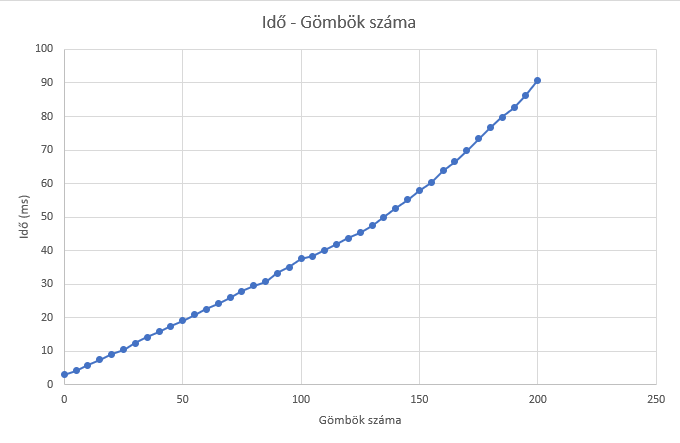
\includegraphics[width=0.8\textwidth,frame]{Test2b}
	\caption{Teljesítményteszt a gömbök számának függvényében}
	\label{fig:Test2}
\end{figure}

Itt is nagyjából lineáris összefüggést tapasztalunk, a labdák számának eggyel való növeléséhez átlagosan 0.4 ms-os növekedés tartozik a kirajzolási időben. Azt tapasztaljuk hogy jóval kevesebb hatása van a gömbök számának növelése a teljesítményre -- kb. $1/7$-e az iterációhoz képest. A tesztkonfigurációnak 100 labda megjelenítse sem okoz problémát, amíg az iterációk száma kelleően alacsonra van állítva.

A gömbök esetében is inkább a megjelenítés okozza a gondot, a \textbf{glDrawArrays()} sor ideiglenes kommentezésével a kirajzolást lényegében megszüntetjük, ám az ütközések modellezését nem befolyásoljuk. Ha ezután újra futtatjuk az előbbi tesztet, akkor megtudhatjuk hogy a fizika kiszámolása mennyire lassította a kirajzolást. A futás eredményének egy részéből készült grafikon \aref{fig:Test3}.~ábrán látható. 

A grafikonra 350-nél kevesebb gömbhöz tartozó mérési értékek nem szerepelnek, az azokhoz tartozó számolási idő kevesebb mint 1 ms volt. Ez jól mutatja hogy a kirajzolási időhöz képest az ütközések kiszámolása jelentéktelen.

\begin{figure}[H]
	\centering
	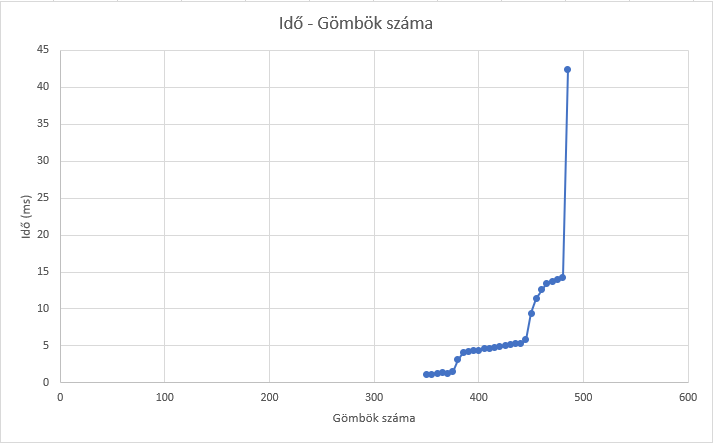
\includegraphics[width=0.8\textwidth,frame]{Test3b}
	\caption{Teljesítményteszt a gömbök számának függvényében, kirajzolás nélkül}
	\label{fig:Test3}
\end{figure}

Az ábra alapján viszont itt már inkább exponenciális összefüggést állapíthatunk meg lineáris helyett. Az utolsó érték 490 gömbbel már 1000 ms volt, de ki lett hagyva az ábrázolás megkönnyítése érdekében. A teszt alatt azonban a magasabb értékek során a processzor összesített kihasználtsága a Windows Task Manager szerint 14\%-os volt, és egyik szál sem mutatott állandó teljes terhelést. 

A fizika futása nem lett több szálra bontva, így nem meglepő hogy csak \textbf{egyetlen processzormagot használ} igazán, azonban az furcsa hogy azt az egyet nem teljes mértékben. A jelenség pontos forrása ismeretlen, könnyen lehet hogy a hardver vagy az operációs rendszer korlátozza biztonsági okokból, ellenben a probléma csak extrém körülmények között jelentkezik, így nem lett sok idő fordítva az ok felkutatására. 

A többi paraméter nincsen mérhető befolyással a teljesítményre. Fontos megjegyezni hogy a kirajzolás módja miatt a kamera pozíciója is befolyásolja a sebességet. Ha egyenesen felfelé nézünk, a sugár lépései jelentősen megnőnek, hiszen mindig a legközelebb lévő felület távolságát lépjük előre, így néhány iteráció elegendő ahhoz hogy kiléphessünk a maximális távolsággal a \textbf{RayMarch()} ciklusából.

Ugyanezen okból kifolyólag a talajtól közel kiinduló, azzal párhuzamos sugarak kis lépésekben tudnak csak haladni, így több iteráció szükséges a \textbf{RayMarch()} ciklusából való kilépéshez, ami lassabb kirajzolási sebességet eredményez.